\documentclass[11pt,a4paper,oneside]{article}
% input the config file
\input{config}

% document begins
\begin{document}

\input{titlepage}
\clearpage

\pagestyle{fancy}
\fancyhead{}
\fancyfoot{}
\fancyfoot[L]{Volume 9 No 2}
\fancyfoot[C]{OCNS Newsletter}
\fancyfoot[R]{Page \thepage}

\clearpage
\pagecolor{ocnspagecolor}
\section*{Message from the President}%
\sectionauthor{Thomas Nowotny, Professor of Informatics, University of Sussex, UK}
\begin{wrapfigure}{l}{0.2\textwidth}
  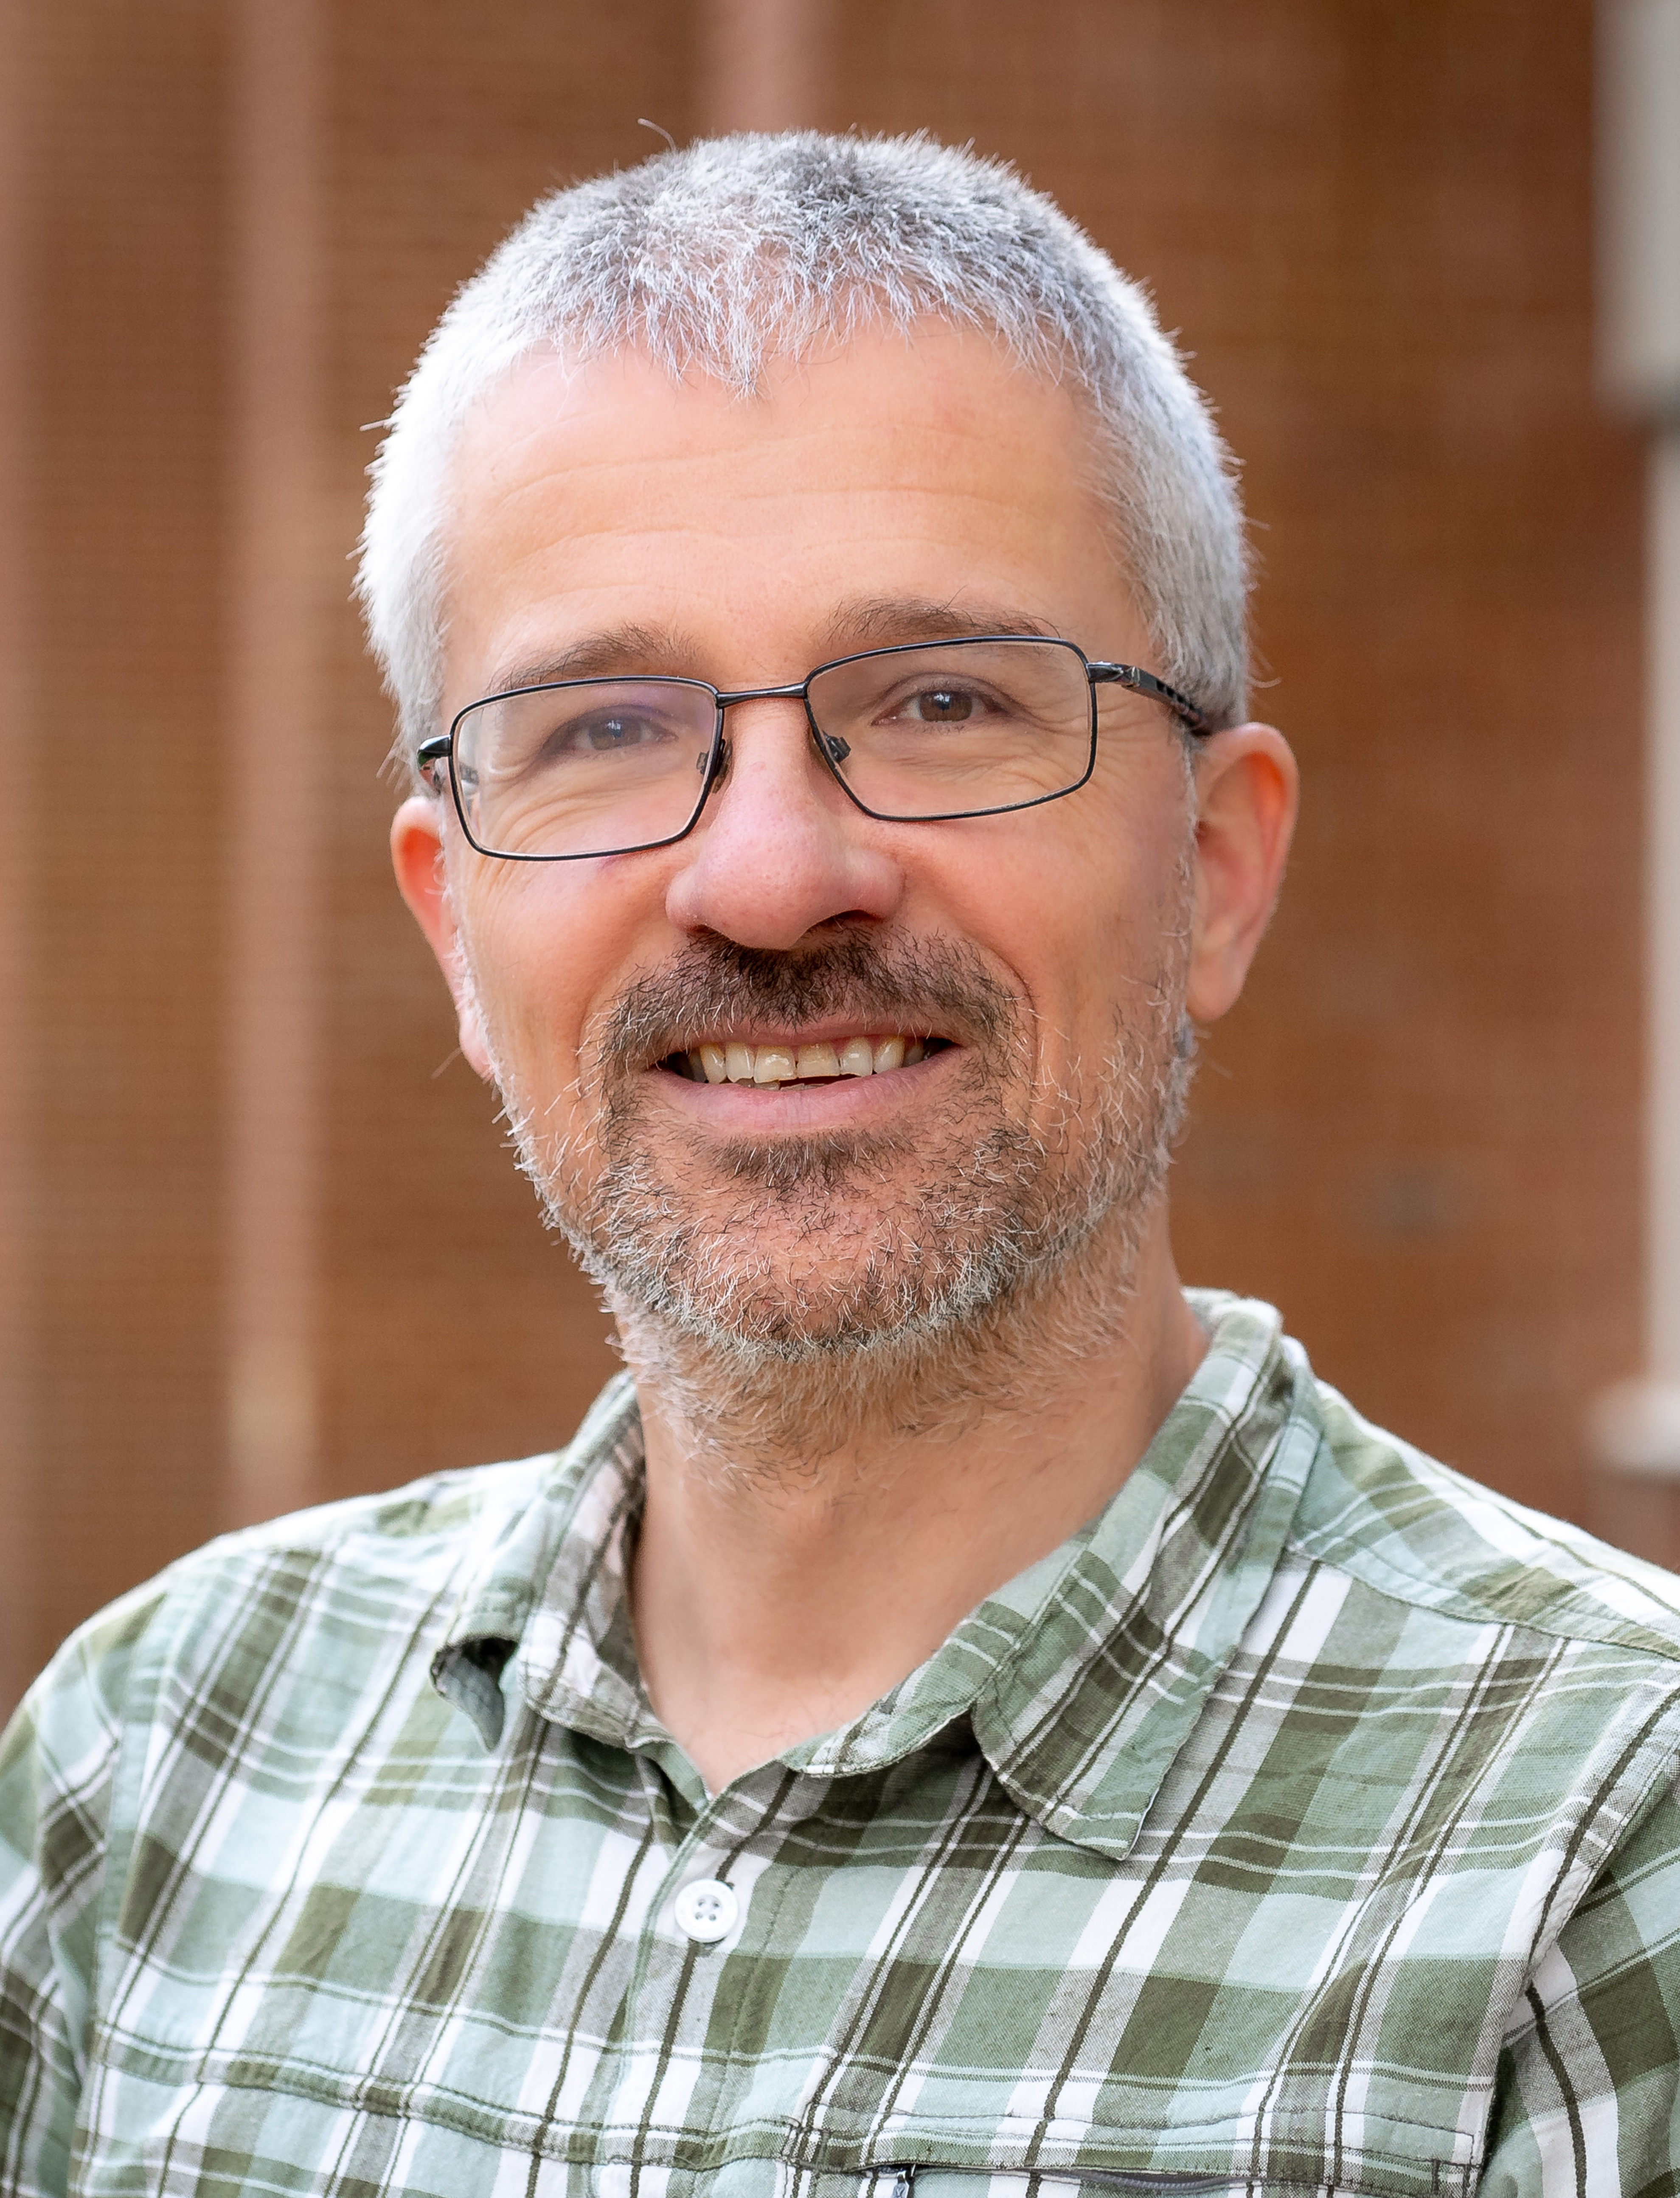
\includegraphics[width=0.2\textwidth]{images/Thomas1}
\end{wrapfigure}

Welcome to the latest edition of our OCNS newsletter.
Last year, the annual CNS conference was held in Florence, the Cradle of the Renaissance.
To fit the bill, we had a well-attended meeting with a lot of scientific energy.
Our thanks go to the local organizers---Michele Migliore, Alessia Bonafede and, most importantly Sergio Solinas.
Equally, many thanks to our Program Committee, led by Julie Haas, and the board of directors, without whose voluntary contributions the CNS conference would not be possible.
You will find more information about the meeting in Florence inside the newsletter.

I would also like to take this opportunity to thank our outgoing directors, Max Garagnani, Dimitrios Pinotsis (Sponsorship chairs), Tatiana Kameneva (Registrations chair), Christopher French (Website/Infrastructure Chair), and Claudio Mirasso (Social Media Chair) for their dedicated service over the last three years.
At the same time, we welcome new board members to continue the operations of OCNS (more inside the newsletter).
Members of the board of directors are appointed through an annual election in the fall, and all OCNS members interested in contributing to the organisation and the CNS meetings are strongly encouraged to apply for election.

Finally, for this year's annual conference, CNS*2026, we return to the North American Continent for the first time since 2018.
We will convene in Halifax, Nova Scotia, Canada, in what is already promising to be another outstanding event.
Tutorial and workshop proposals are looking strong, and registration is open!
I am looking forward to seeing many of you at the Halifax Convention Centre in July.

\vspace{2ex}

\section*{In this issue}%
\sectionauthor{\vspace{-5ex}}
\textcolor{BlueViolet}{%
  \Large
    \begin{itemize}
      \item Announcing CNS*2026 in Halifax
      \item Updates from CNS*2025 Florence
      %\item Updates from OCNS initiatives
      %\item Updates from OCNS Members
    \end{itemize}
}

\vspace{2ex}
\centerline{\rule{0.5\textwidth}{0.4pt}}
\iffalse{}
\vspace{1ex}
\begin{center}
\begin{tcolorbox}[colback=lighterOrange, colframe=black, width=0.9\textwidth, boxrule=0.1mm]
See pictures from CNS*2025 Florence here: \url{https://www.cnsorg.org/cns-2025-photo-album}.
\end{tcolorbox}
\end{center}
\vspace{1ex}
\centerline{\rule{0.5\textwidth}{0.4pt}}
\vspace{1ex}
\fi{}

\clearpage
\section*{CNS*2026: Halifax, Canada July 11--15, 2026}%
\sectionauthor{%
  \hspace{-1ex}\begin{tabularx}{\textwidth}{lX}%
    Local Organizers: & Thomas Trappenberg, Dalhousie University, Canada\\
  \end{tabularx}}

\begin{figure}[ht]
  \centering
  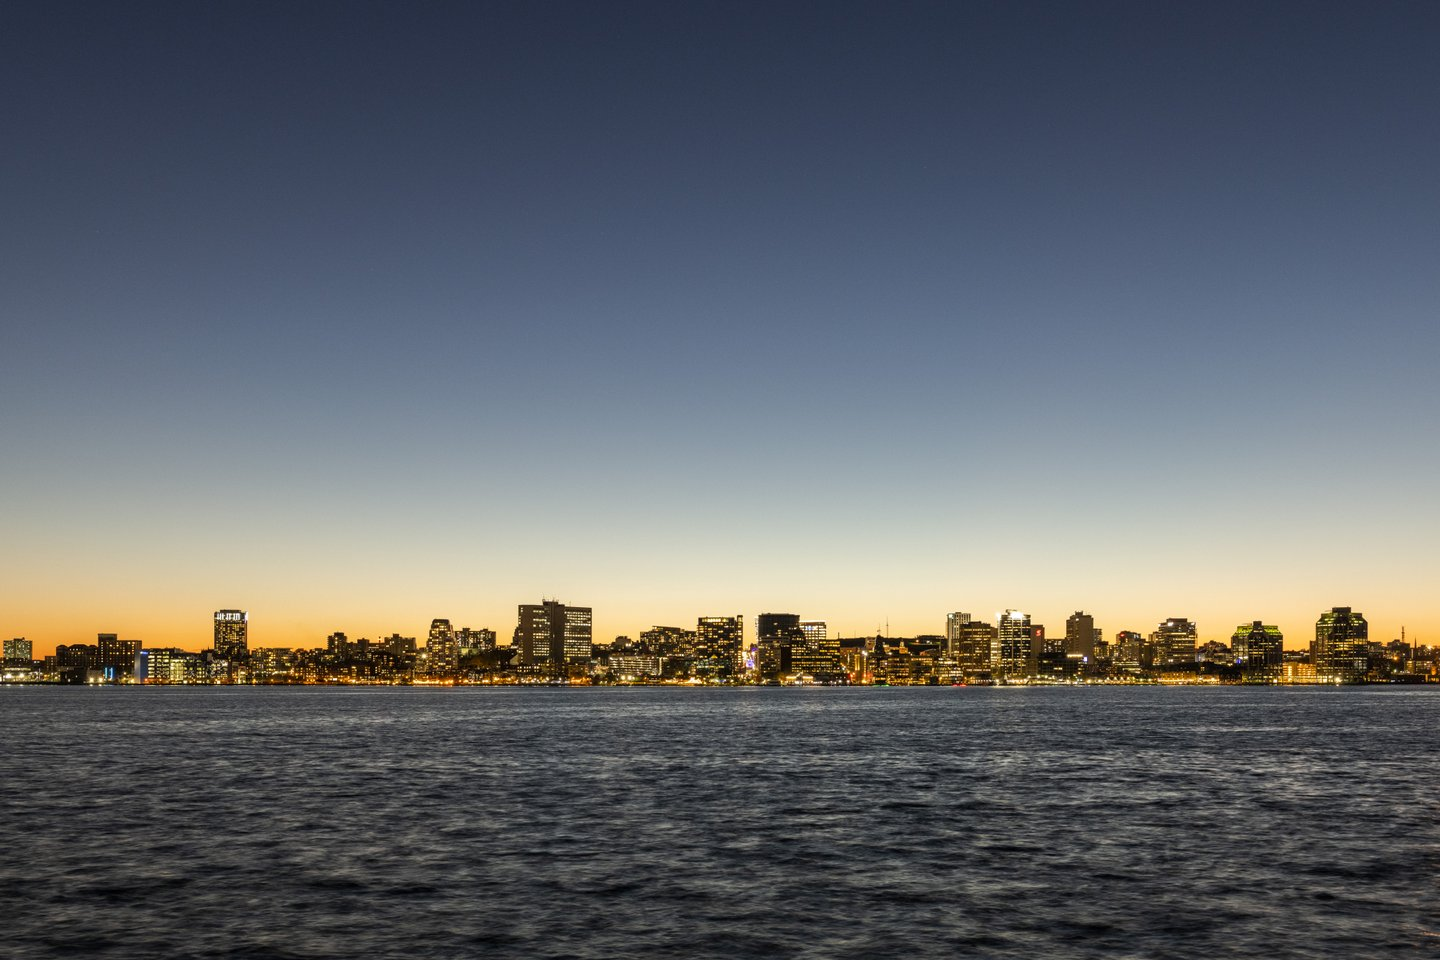
\includegraphics[width=\textwidth]{images/halifax-2}
\end{figure}

%\begin{center}
%\textcolor{Blue}{\textbf{\Large Halifax: }}
%\end{center}

\vspace{1ex}
\centerline{\rule{0.5\textwidth}{0.4pt}}
\vspace{1ex}
\begin{center}
  \textcolor{Blue}{\textbf{\Large OCNS is excited to invite you to the\\\vspace{2ex}35th Annual Computational Neuroscience meeting\\\vspace{2ex}CNS*2026\\\vspace{2ex}{in}\\\vspace{2ex}Halifax, Canada from July 11--15, 2026.}}
\end{center}
\vspace{1ex}
\centerline{\rule{0.5\textwidth}{0.4pt}}
\vspace{2ex}
\begin{center}
\textcolor{Blue}{\textbf{\Large Registration and abstract submission is open!}}
\end{center}
\vspace{1ex}
\centerline{\rule{0.5\textwidth}{0.4pt}}
\vspace{2ex}
\begin{center}
\begin{tcolorbox}[colback=lighterOrange, colframe=black, width=0.45\textwidth, boxrule=0.1mm]
\begin{center}
\href{https://www.cnsorg.org/cns-2026-quick}{https://www.cnsorg.org/cns-2026-quick}.
\end{center}
\end{tcolorbox}
\end{center}

\clearpage
%\section*{OCNS Board:\ Elections: Nominations are open!}%
\sectionauthor{
  \hspace{-1ex}\begin{tabularx}{\textwidth}{lX}%
    2024 Nomination Committee: & Shailesh Appukuttan, Aix-Marseille University, France (Chair)\\
    & Christopher French, University Of Melbourne, Australia\\
    & Robert McDougal, Yale University, USA \\
    & Eirini Mavritsaki, Birmingham City University, UK \\
  \end{tabularx}}%

The nomination period for self-nominations for the election of new members of the \href{https://www.cnsorg.org/board-of-directors}{OCNS Board of Directors} is now open.
New Directors will serve a three-year term from January 2025 through December 2027 and will initially fill the following roles:
\begin{multicols}{2}
  \begin{itemize}
    \item \textbf{Registration Chair}
    \item \textbf{Sponsorship Chair}
  \end{itemize}
\end{multicols}

New Directors will act as Deputy Chairs in their roles by shadowing the current Chairs for a year, and then will take over when the current Chairs finish their terms.
Candidates need to be current OCNS members and are required to have been OCNS members for at least a year or to attend an on-site CNS conference in the past.
More information about the new Directors' election can be found at:
\vspace{2ex}
\begin{center}
\url{https://www.cnsorg.org/election-procedures}
\end{center}
\vspace{2ex}

We encourage OCNS members to consider self-nomination for these elections.

%\begin{tcolorbox}[colback=lighterOrange, colframe=black, width=\textwidth, boxrule=0.1mm, leftrule=0.1mm, rightrule=0mm]
\begin{tcolorbox}[colback=lighterOrange, colframe=black, width=\textwidth, boxrule=0.1mm]
\textbf{OCNS is committed to have a wide diversity among its Directors---across research areas, gender, abilities, career experiences, geographic locations, and personal backgrounds.
OCNS strives to be a diverse group and encourages a balanced and inclusive representation of women in leadership positions within the organization.
This is possible only if a broad range of members apply.}\\\vspace{1ex}

\textbf{We strongly encourage members from under-represented groups to apply, to help OCNS achieve a better representation of the diversity within our scientific community.}
\end{tcolorbox}

Please contact our EDI Chair Eirini Mavritsaki (\href{mailto:eirini.mavritsaki@bcu.ac.uk}{eirini.mavritsaki@bcu.ac.uk}) if you wish to have a short informational meeting about joining the board.

To apply, please use the form:
\vspace{2ex}
\begin{center}
\url{https://www.cnsorg.org/board-nomination-2024}
\end{center}

\vspace{2ex}
\textbf{The extended deadline for application is \underline{October 21, 2024}.}

\vspace{4ex}

\section*{OCNS Board:\ 2026}%
\sectionauthor{\vspace{-4ex}}

\vfill{}

\begin{figure}[h]
  \begin{center}
  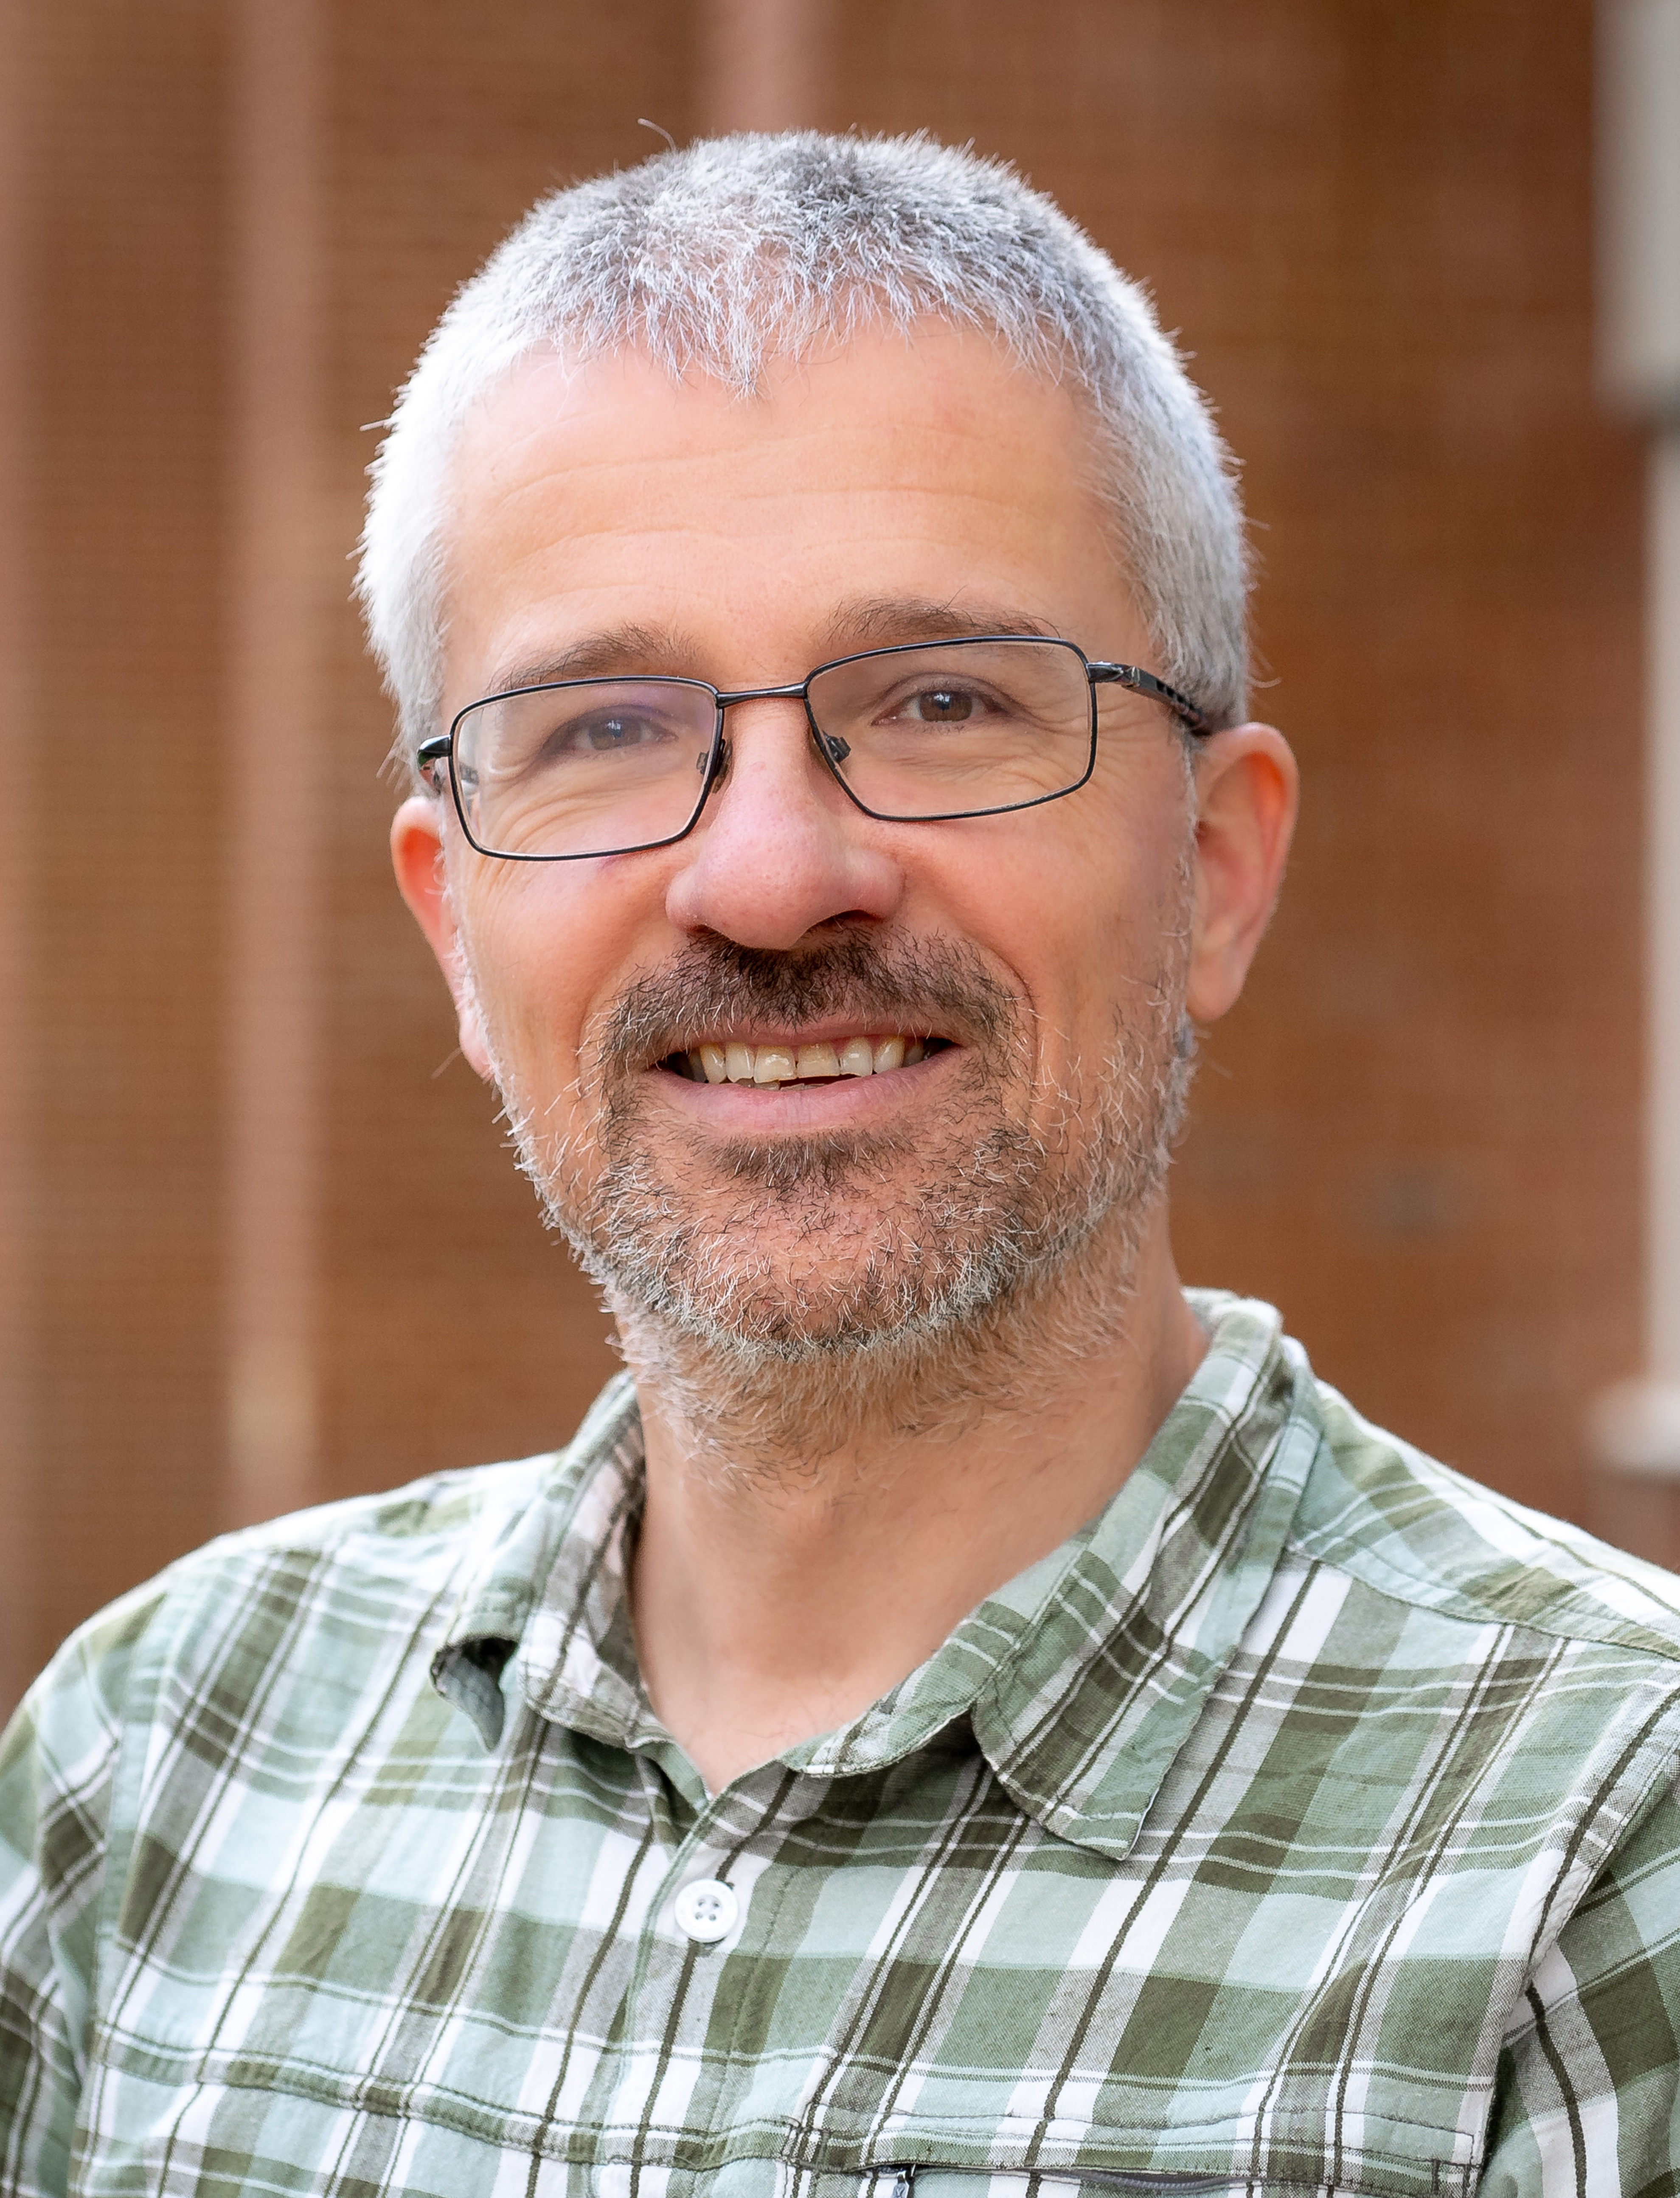
\includegraphics[height=16ex]{images/Thomas1}%
  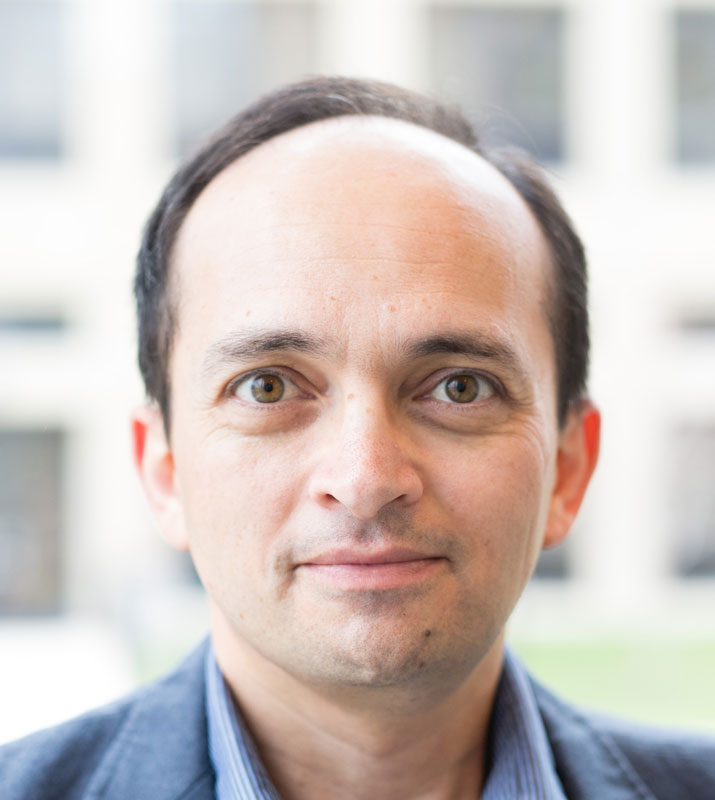
\includegraphics[height=16ex]{images/Rubchinsky}%
  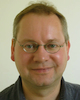
\includegraphics[height=16ex]{images/volker}%
  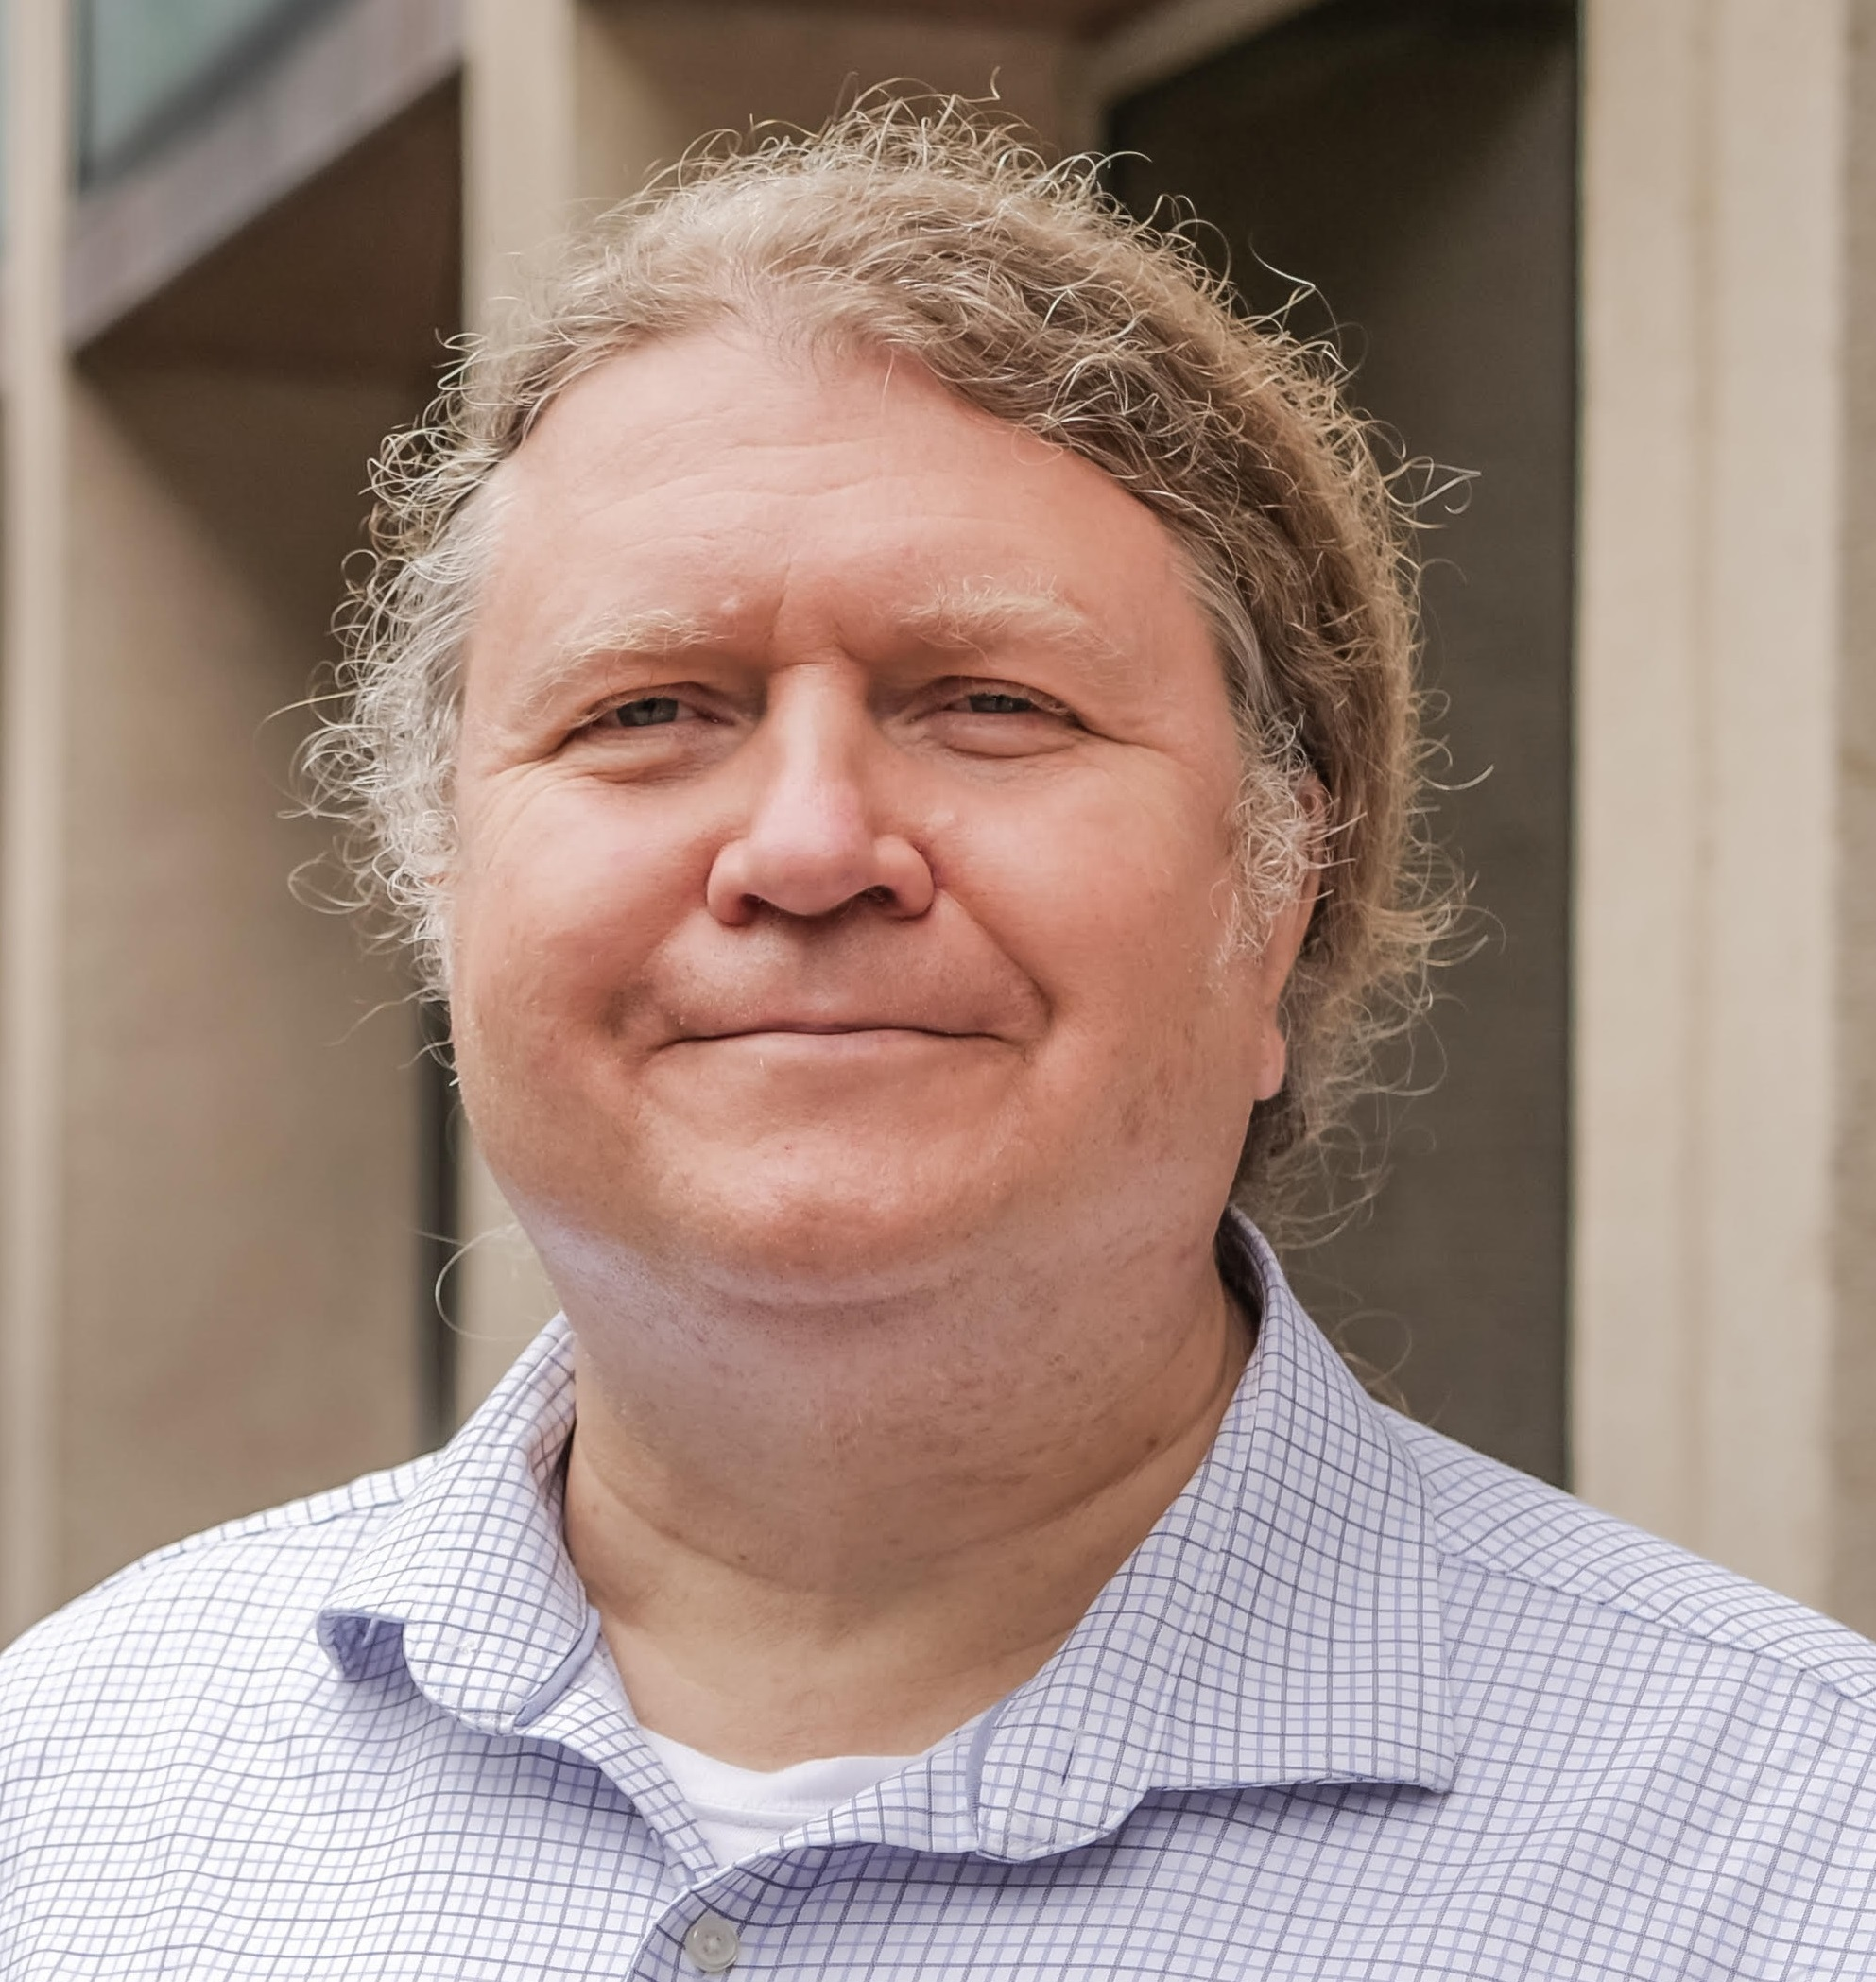
\includegraphics[height=16ex]{images/Cymbalyuk}%
  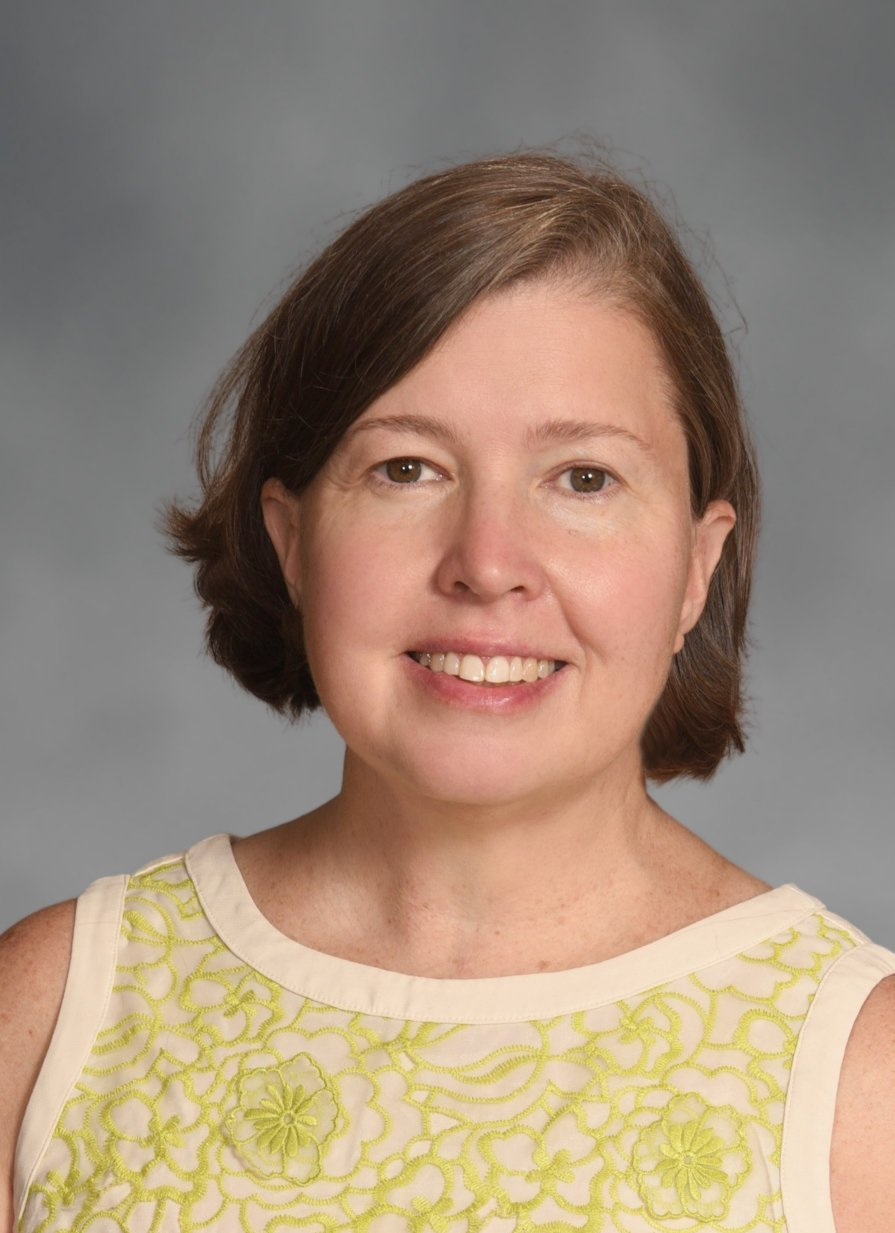
\includegraphics[height=16ex]{images/Haas}\\
  %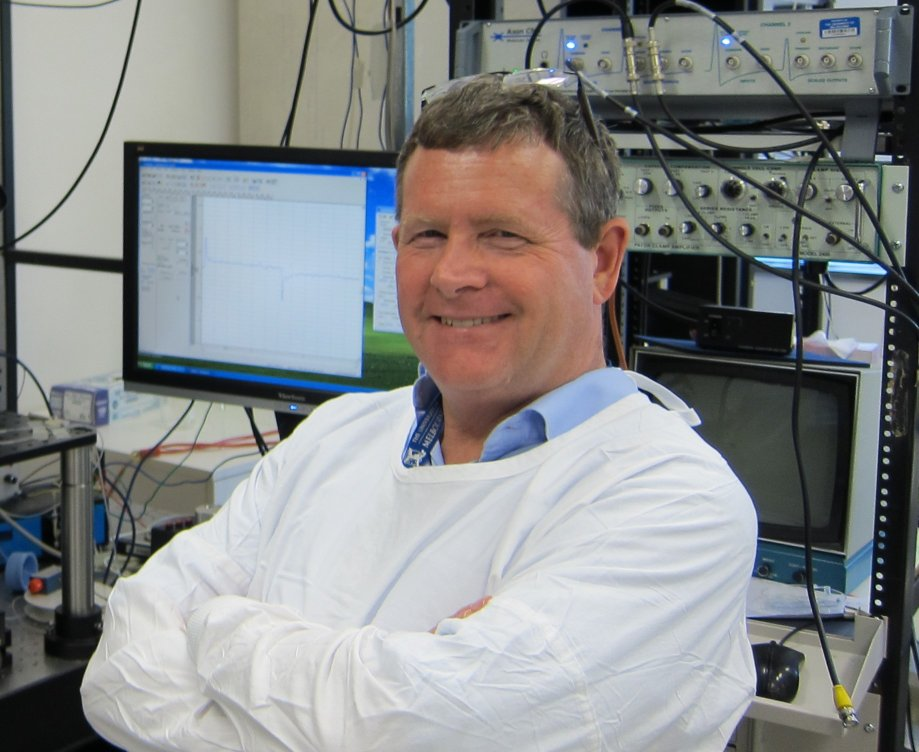
\includegraphics[height=16ex]{images/French}%
  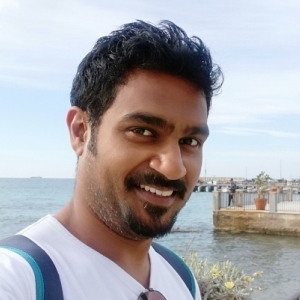
\includegraphics[height=16ex]{images/Shailesh_Appukuttan_square}%
  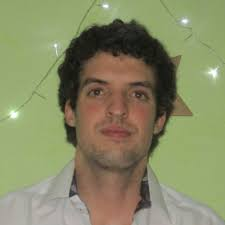
\includegraphics[height=16ex]{images/Baravalle}%
  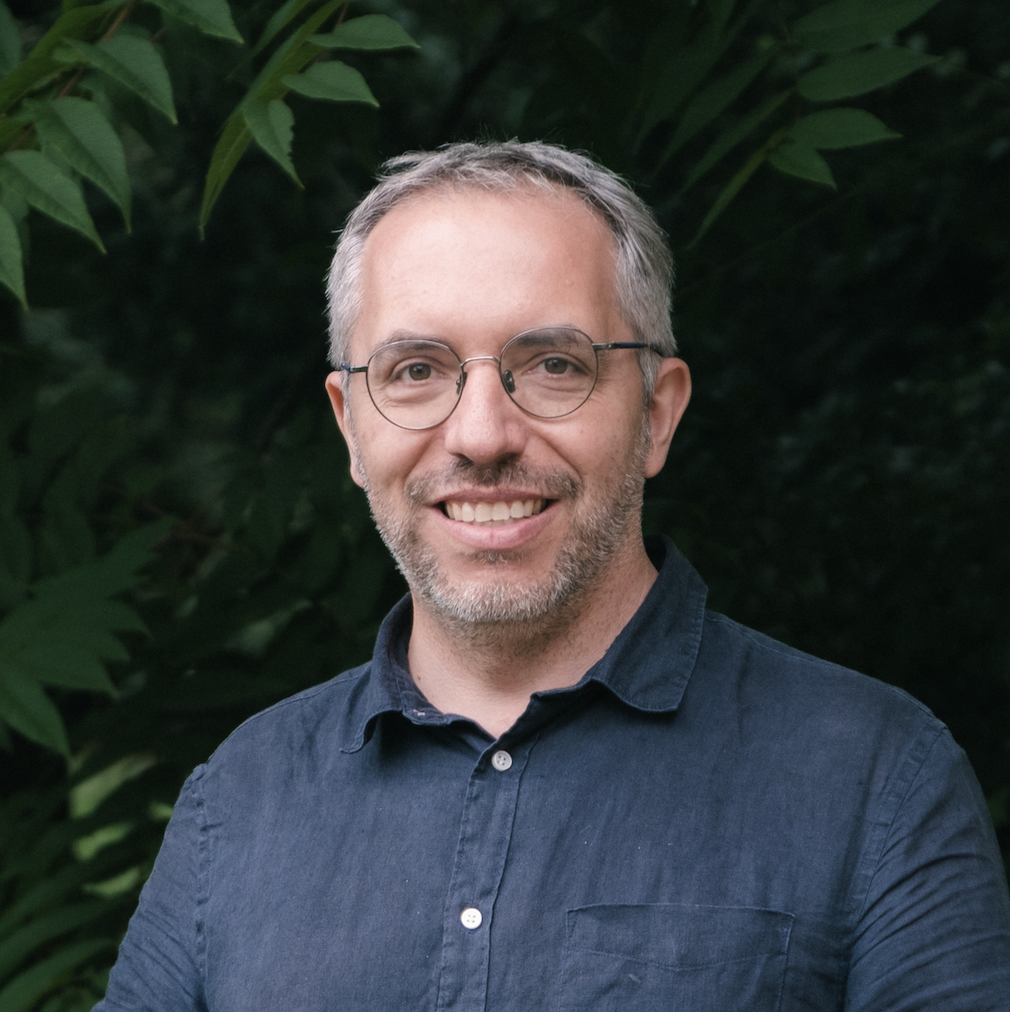
\includegraphics[height=16ex]{images/Battaglia}%
  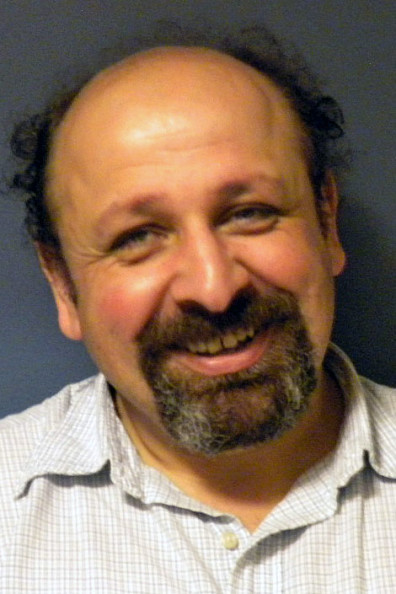
\includegraphics[height=16ex]{images/Dimitrov}%
  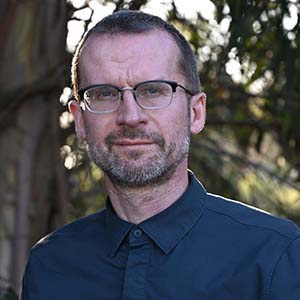
\includegraphics[height=16ex]{images/Janusonis}\\%
  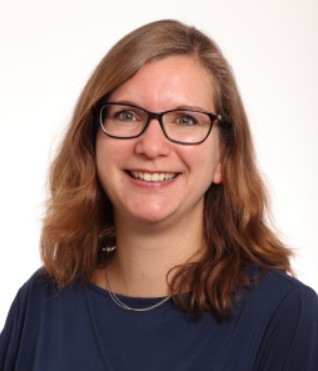
\includegraphics[height=16ex]{images/kerstin}%
  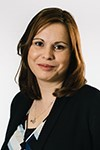
\includegraphics[height=16ex]{images/Mavritsaki}%
  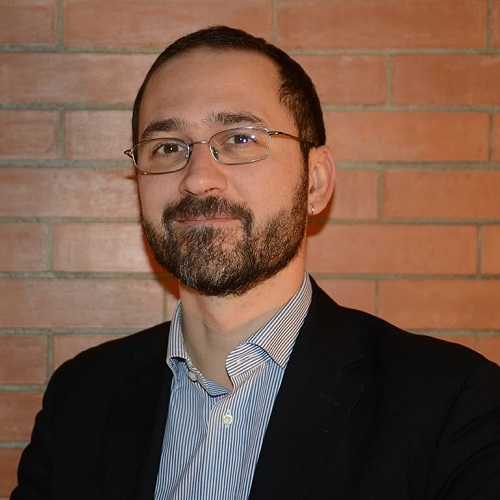
\includegraphics[height=16ex]{images/Mazzoni}%
  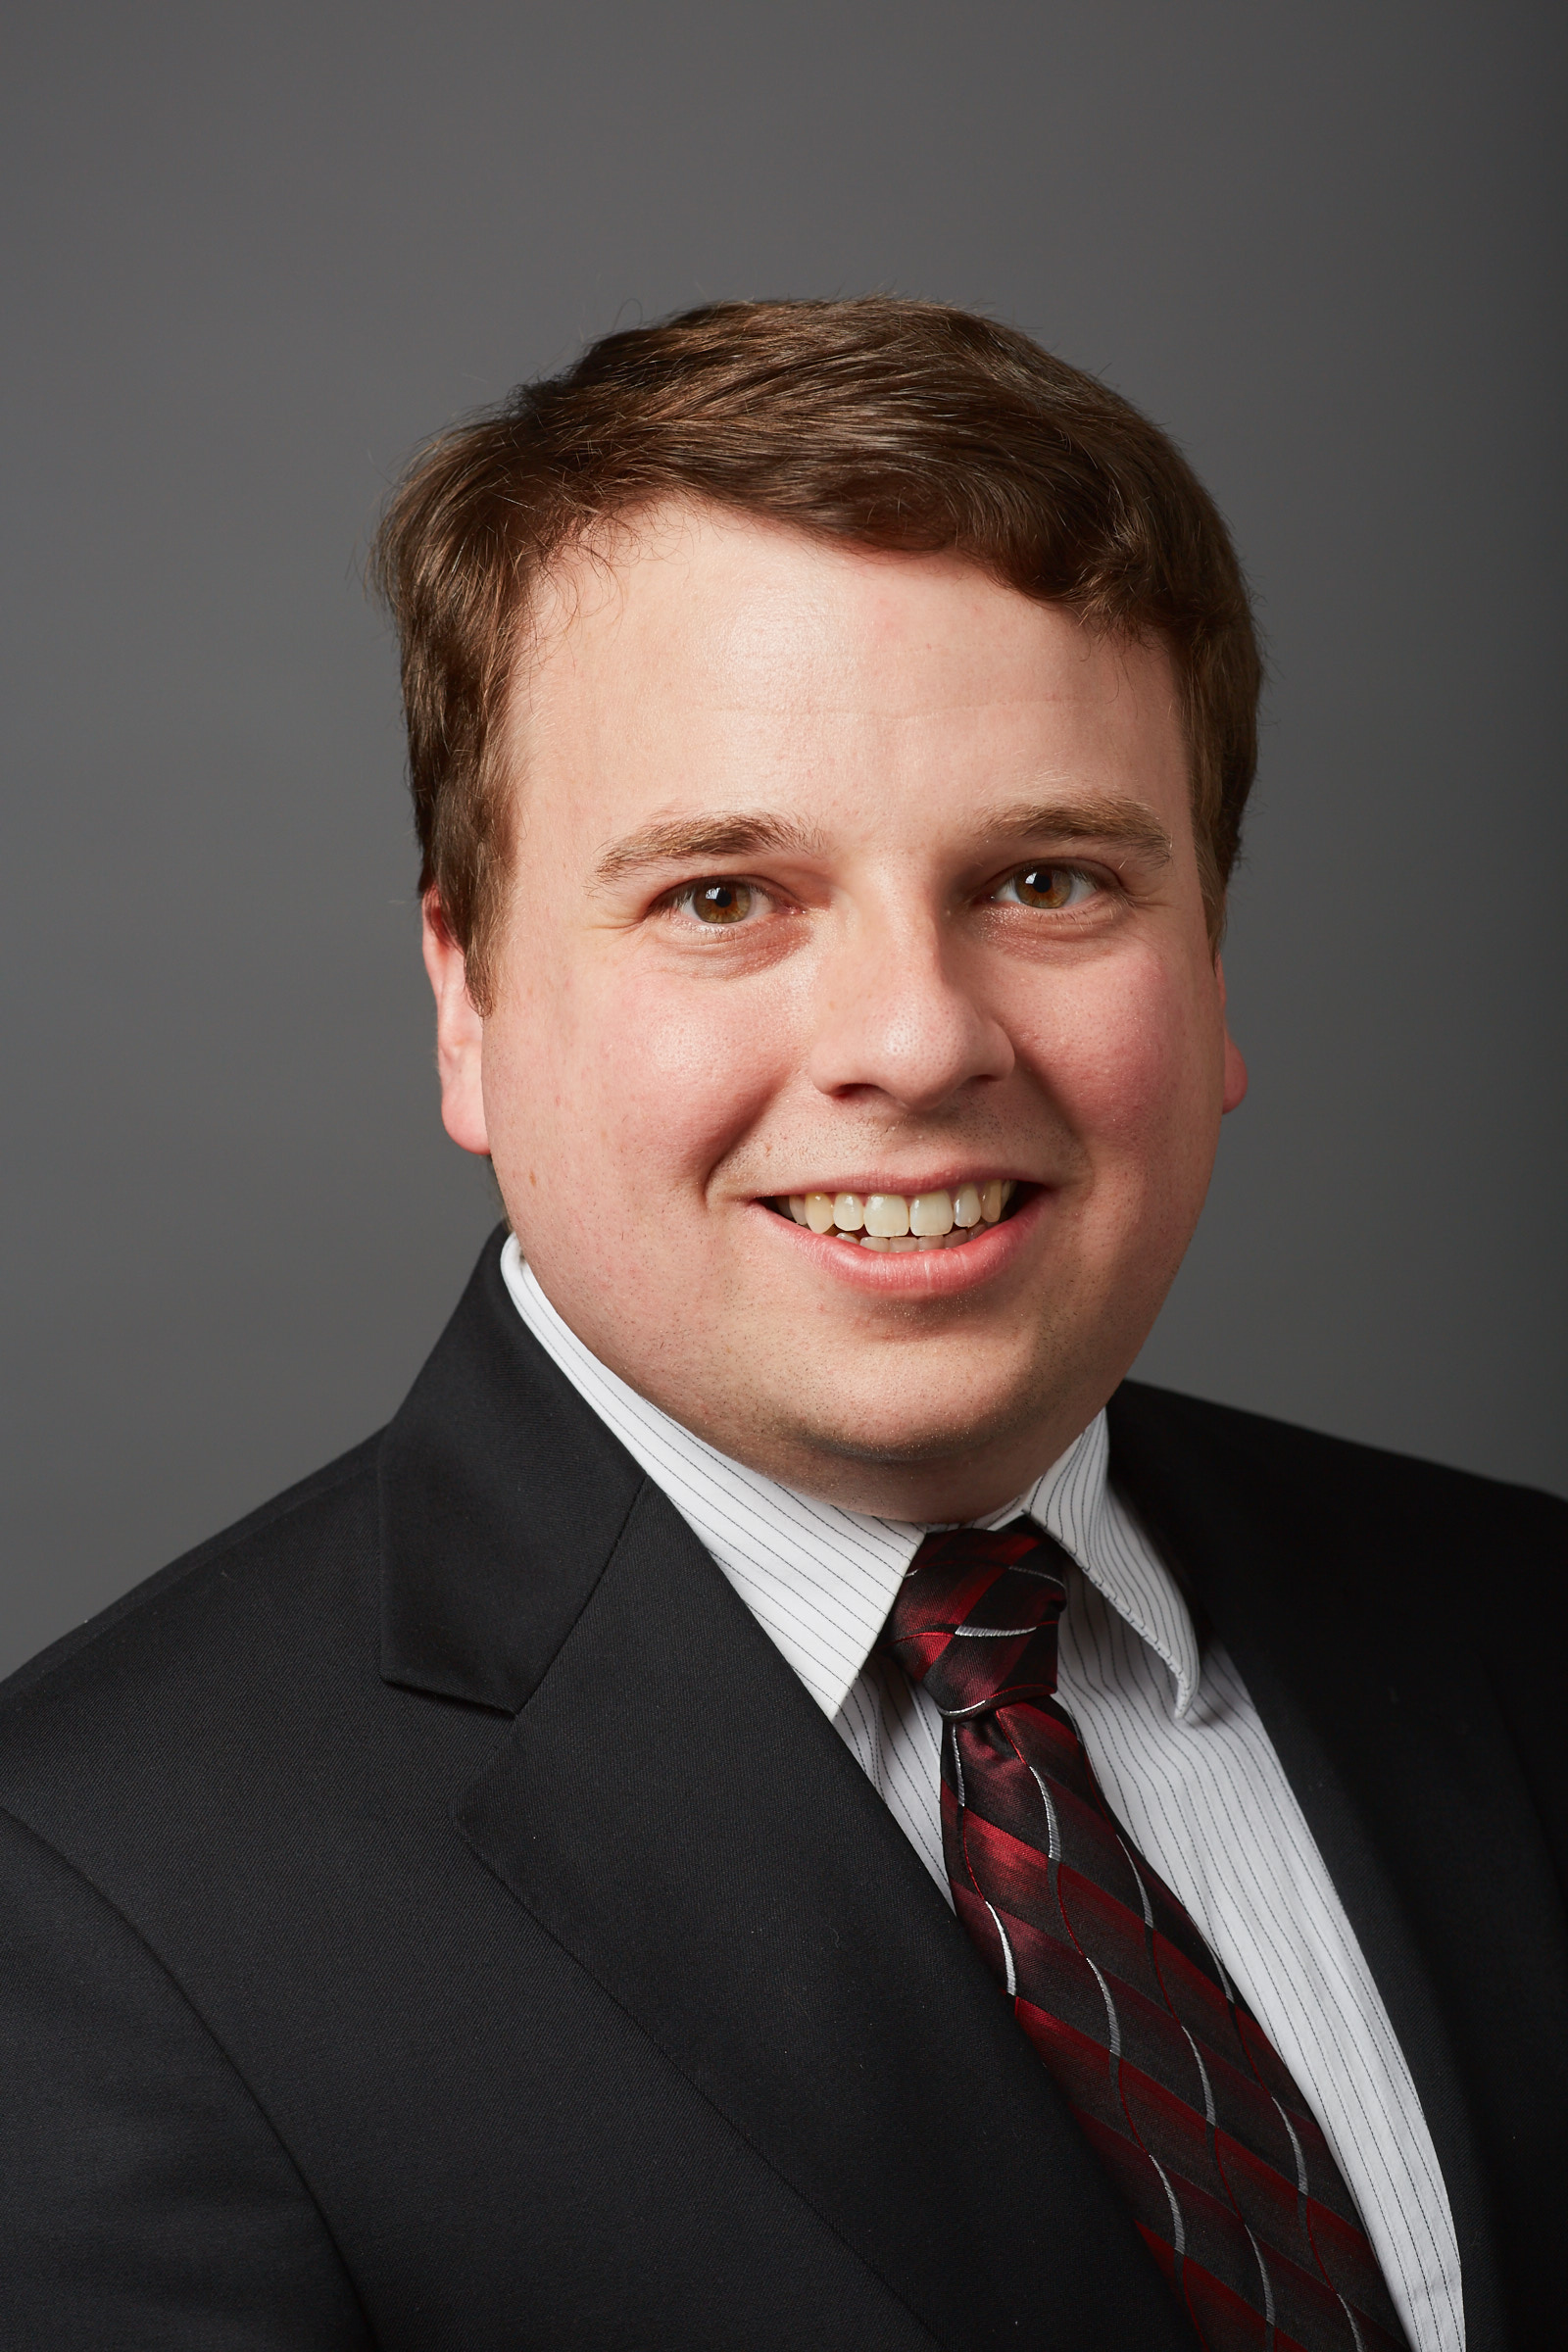
\includegraphics[height=16ex]{images/Robert_McDougal}
  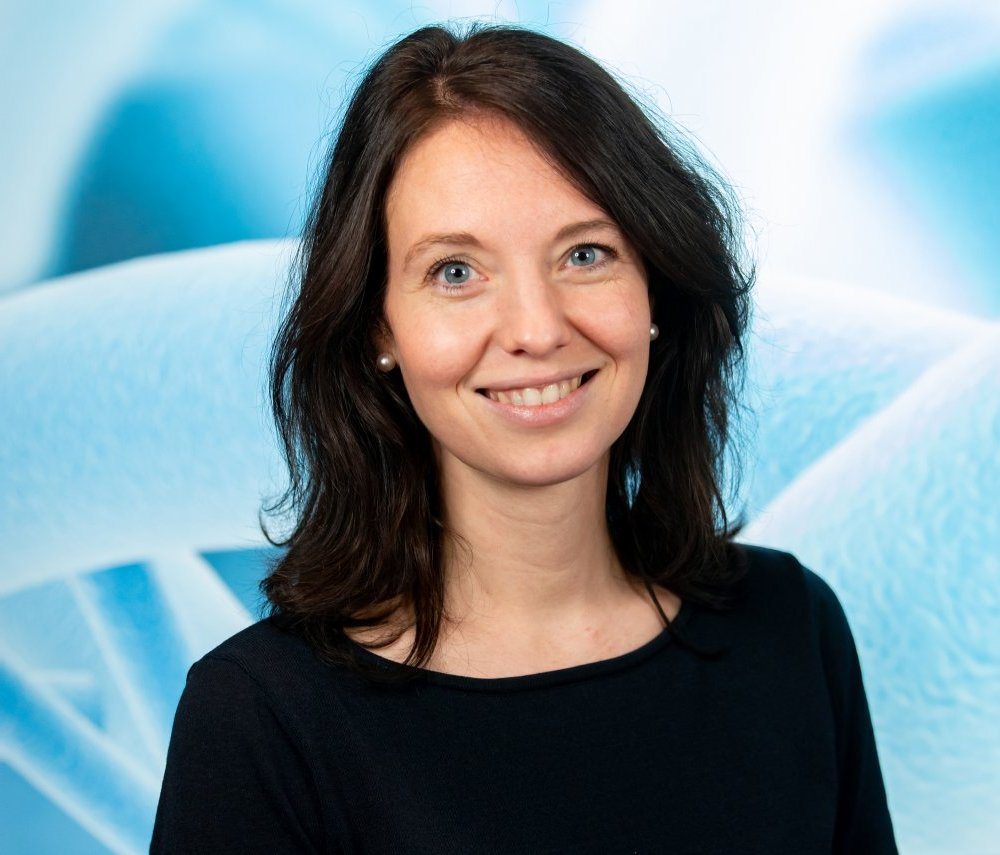
\includegraphics[height=16ex]{images/Moerel}\\%
  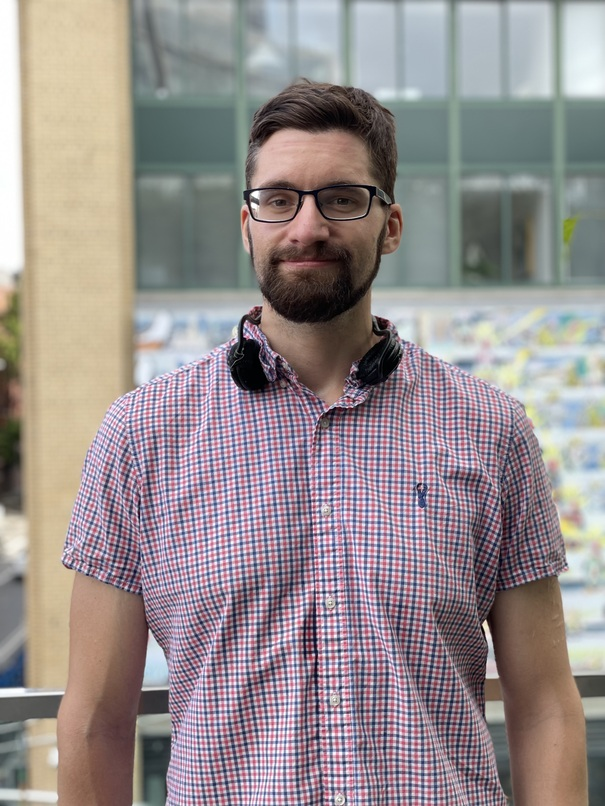
\includegraphics[height=16ex]{images/Newton}%
  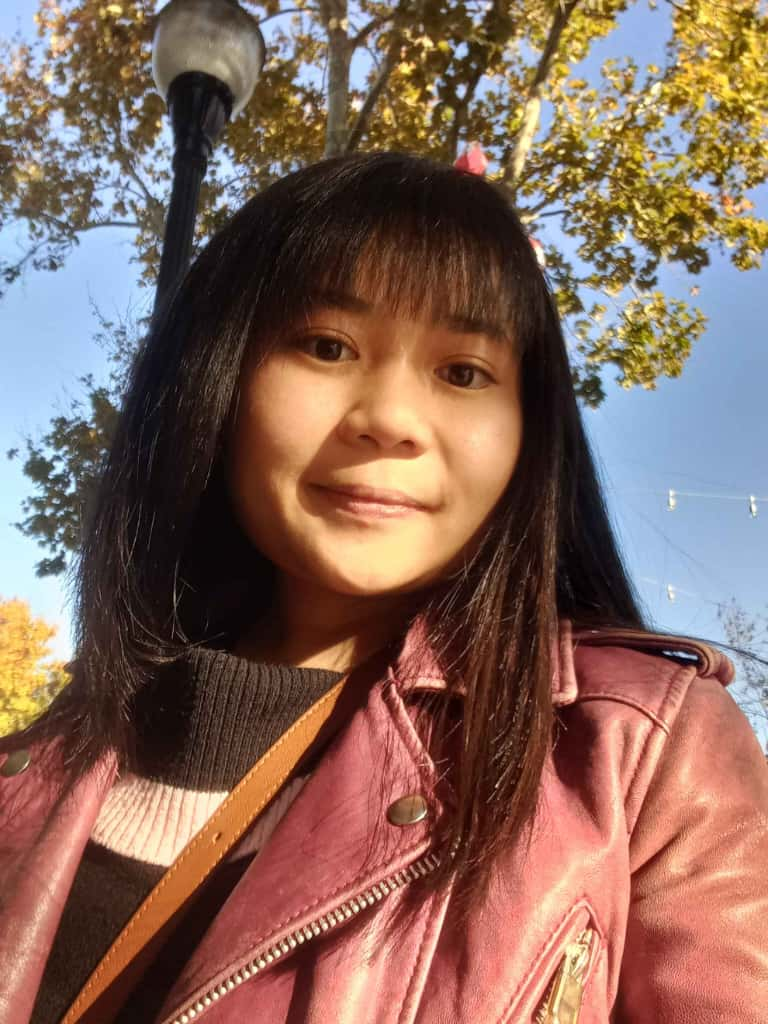
\includegraphics[height=16ex]{images/Nghiem}%
  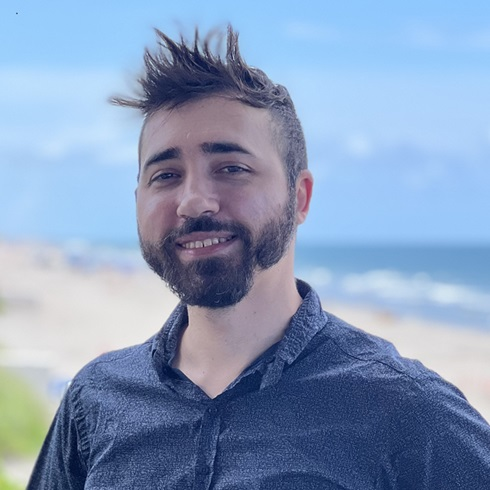
\includegraphics[height=16ex]{images/rodrigo}%
  
\includegraphics[height=16ex]{images/Papoutsi}%
  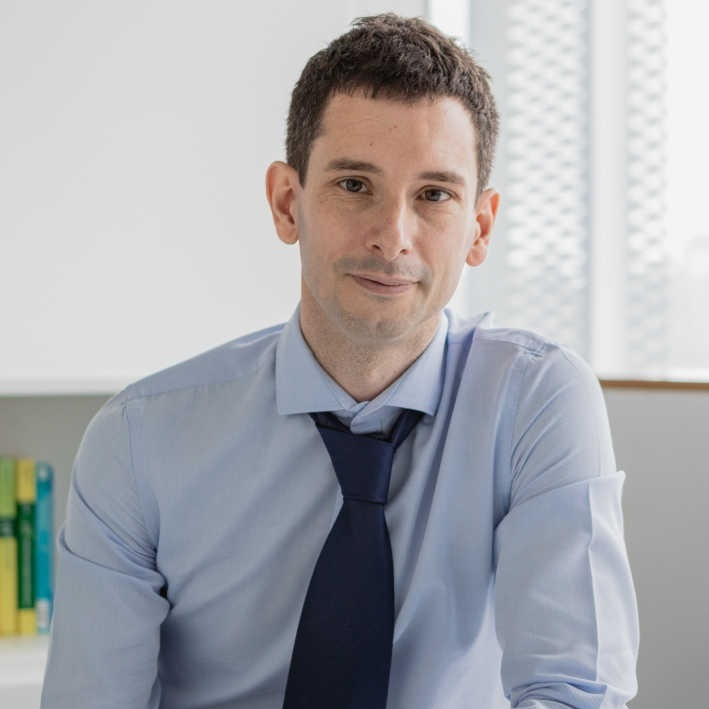
\includegraphics[height=16ex]{images/Pitta}\\%
  
\includegraphics[height=16ex]{images/Cesar}%
  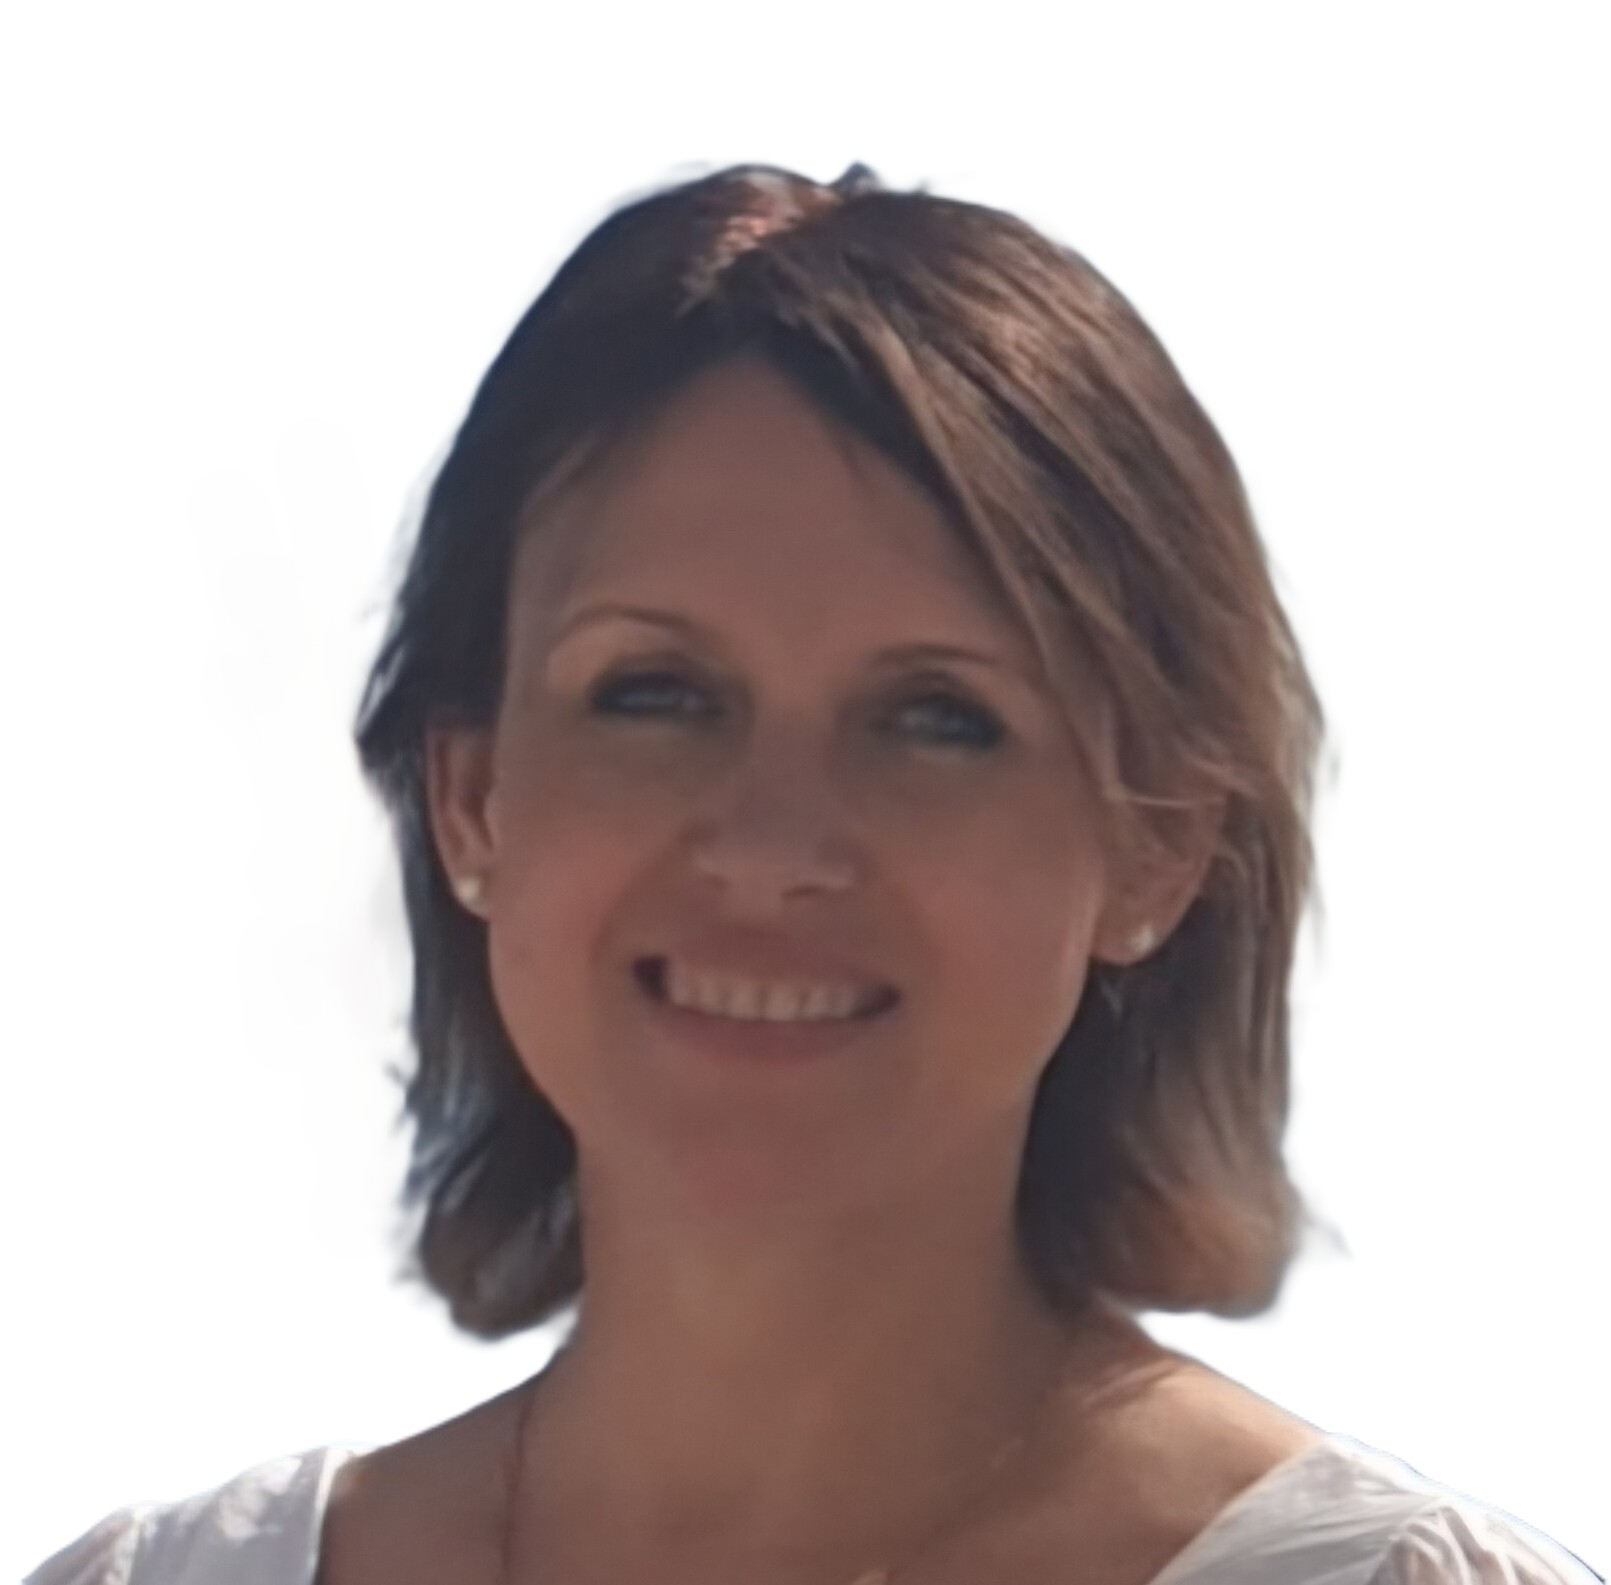
\includegraphics[height=16ex]{images/Saudargiene}%
  
\includegraphics[height=16ex]{images/ankur-sinha}%
  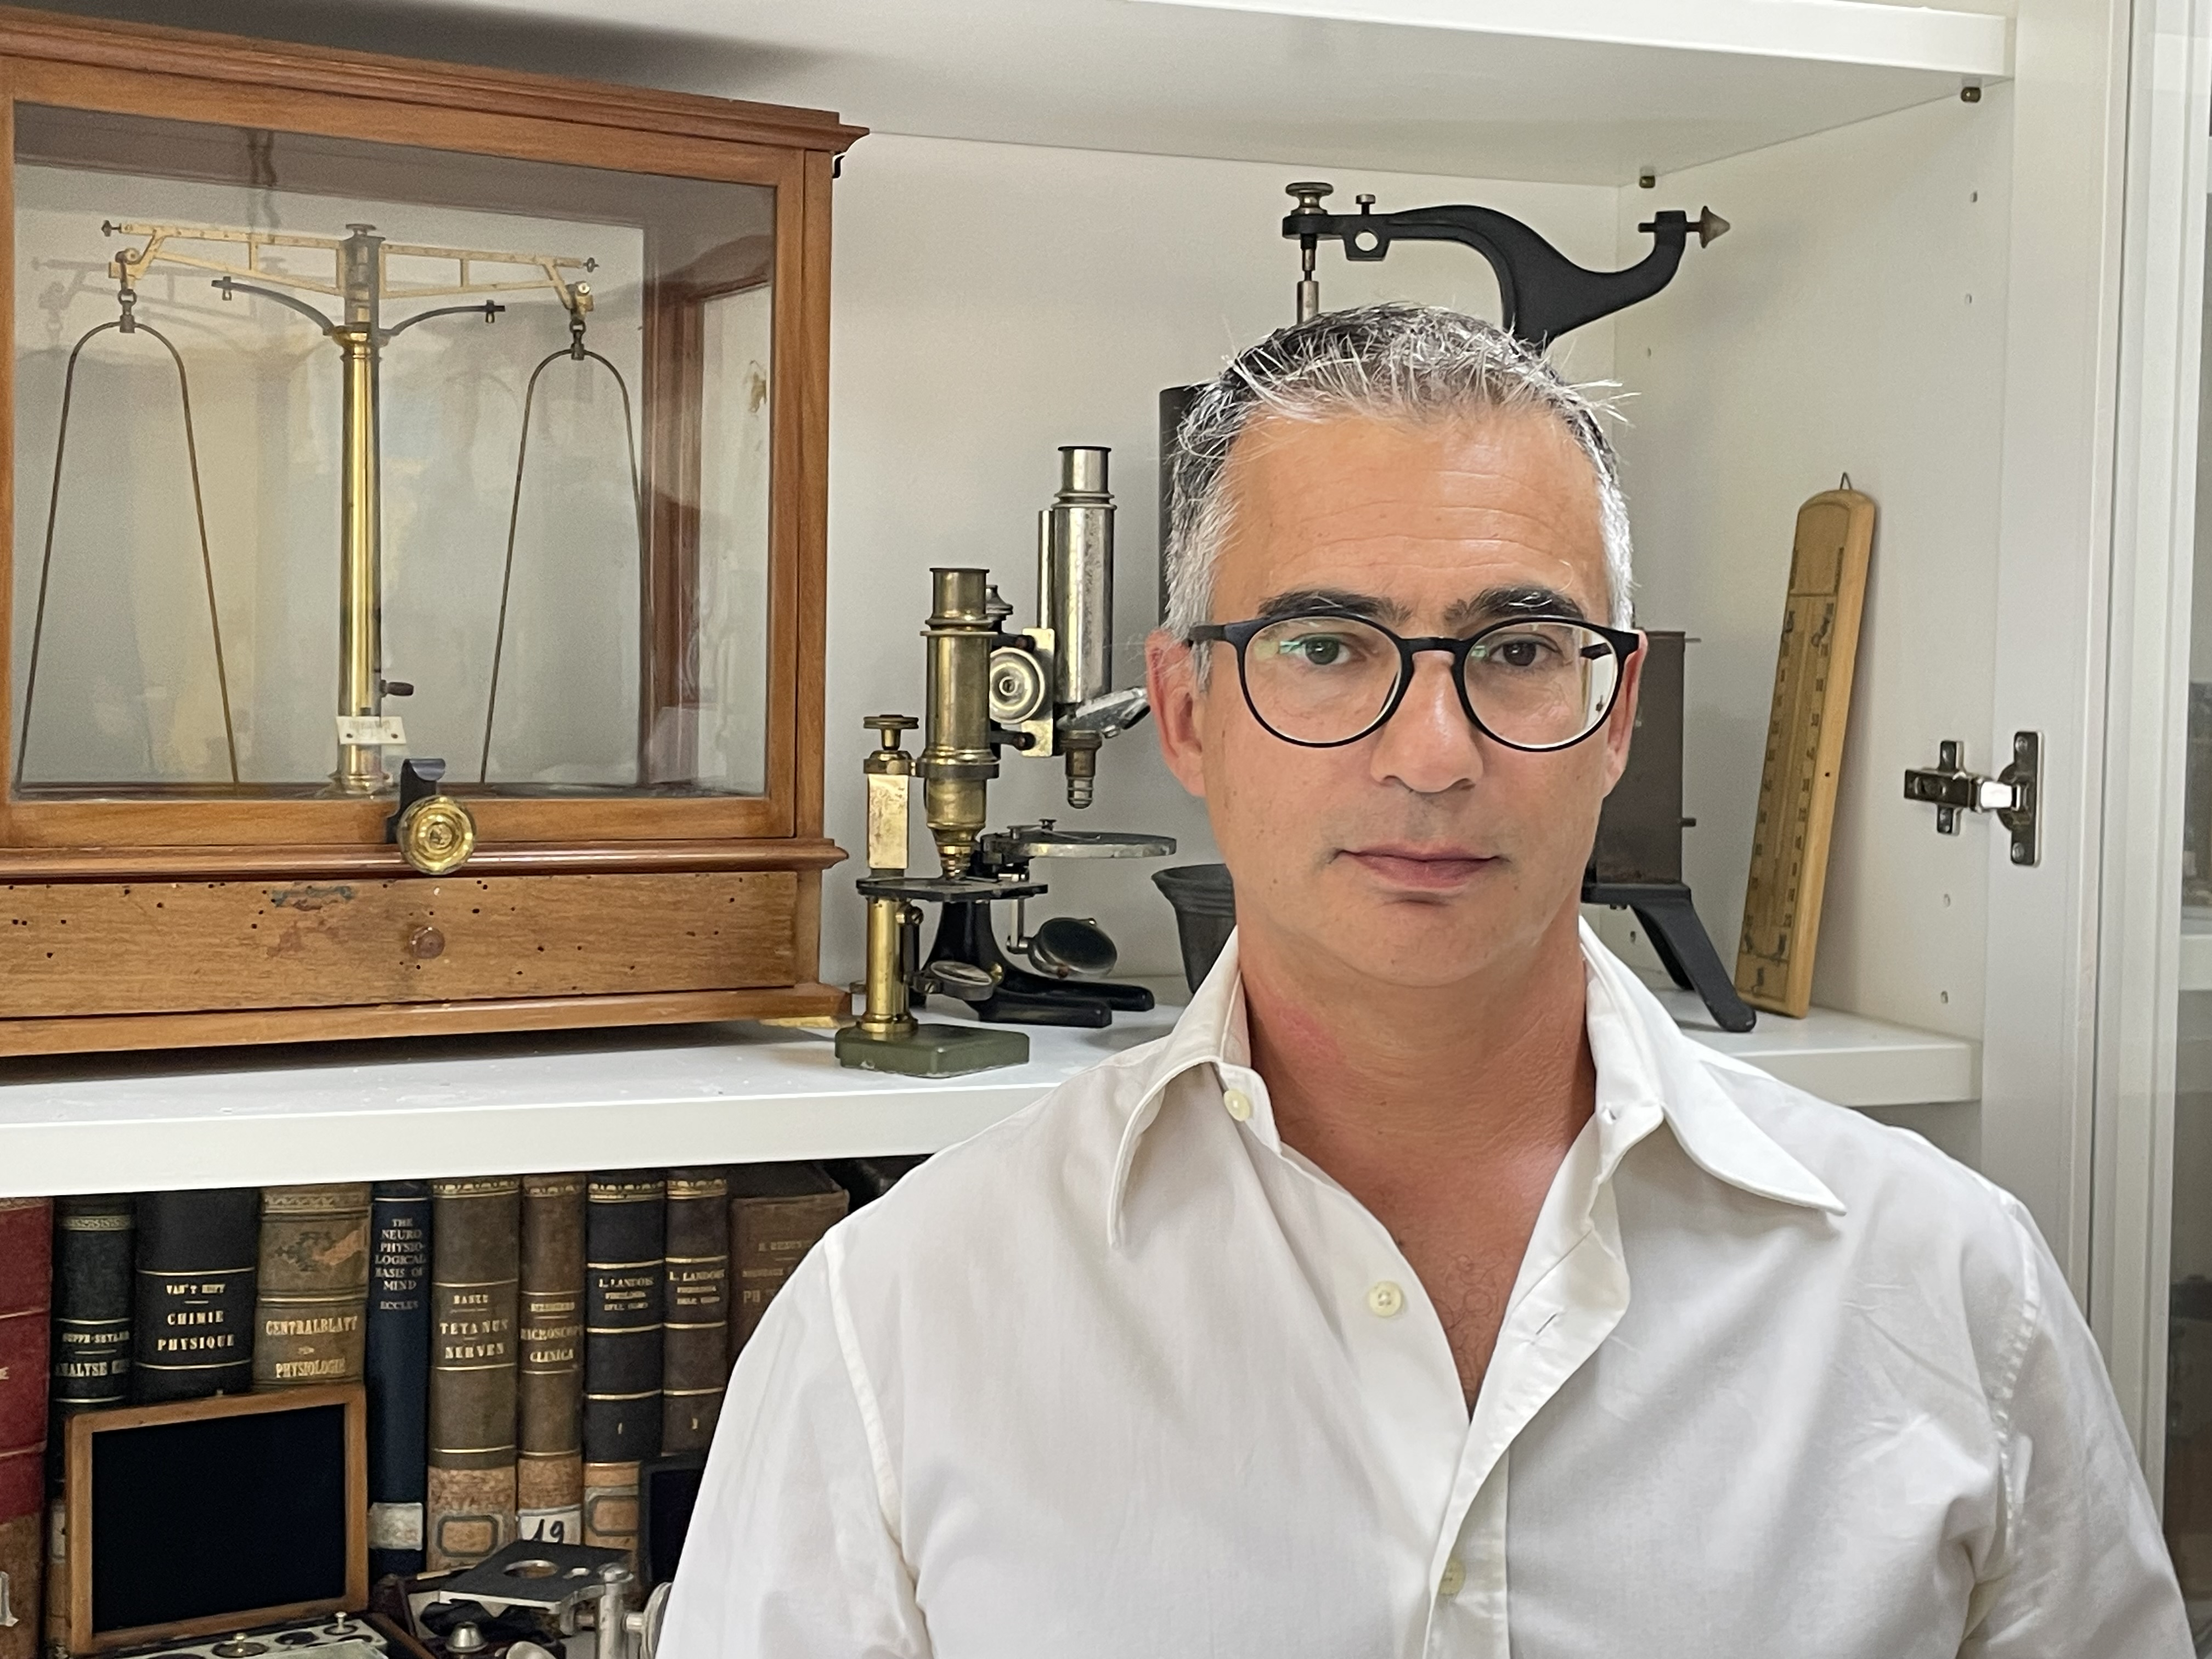
\includegraphics[height=16ex]{images/Solinas}%
  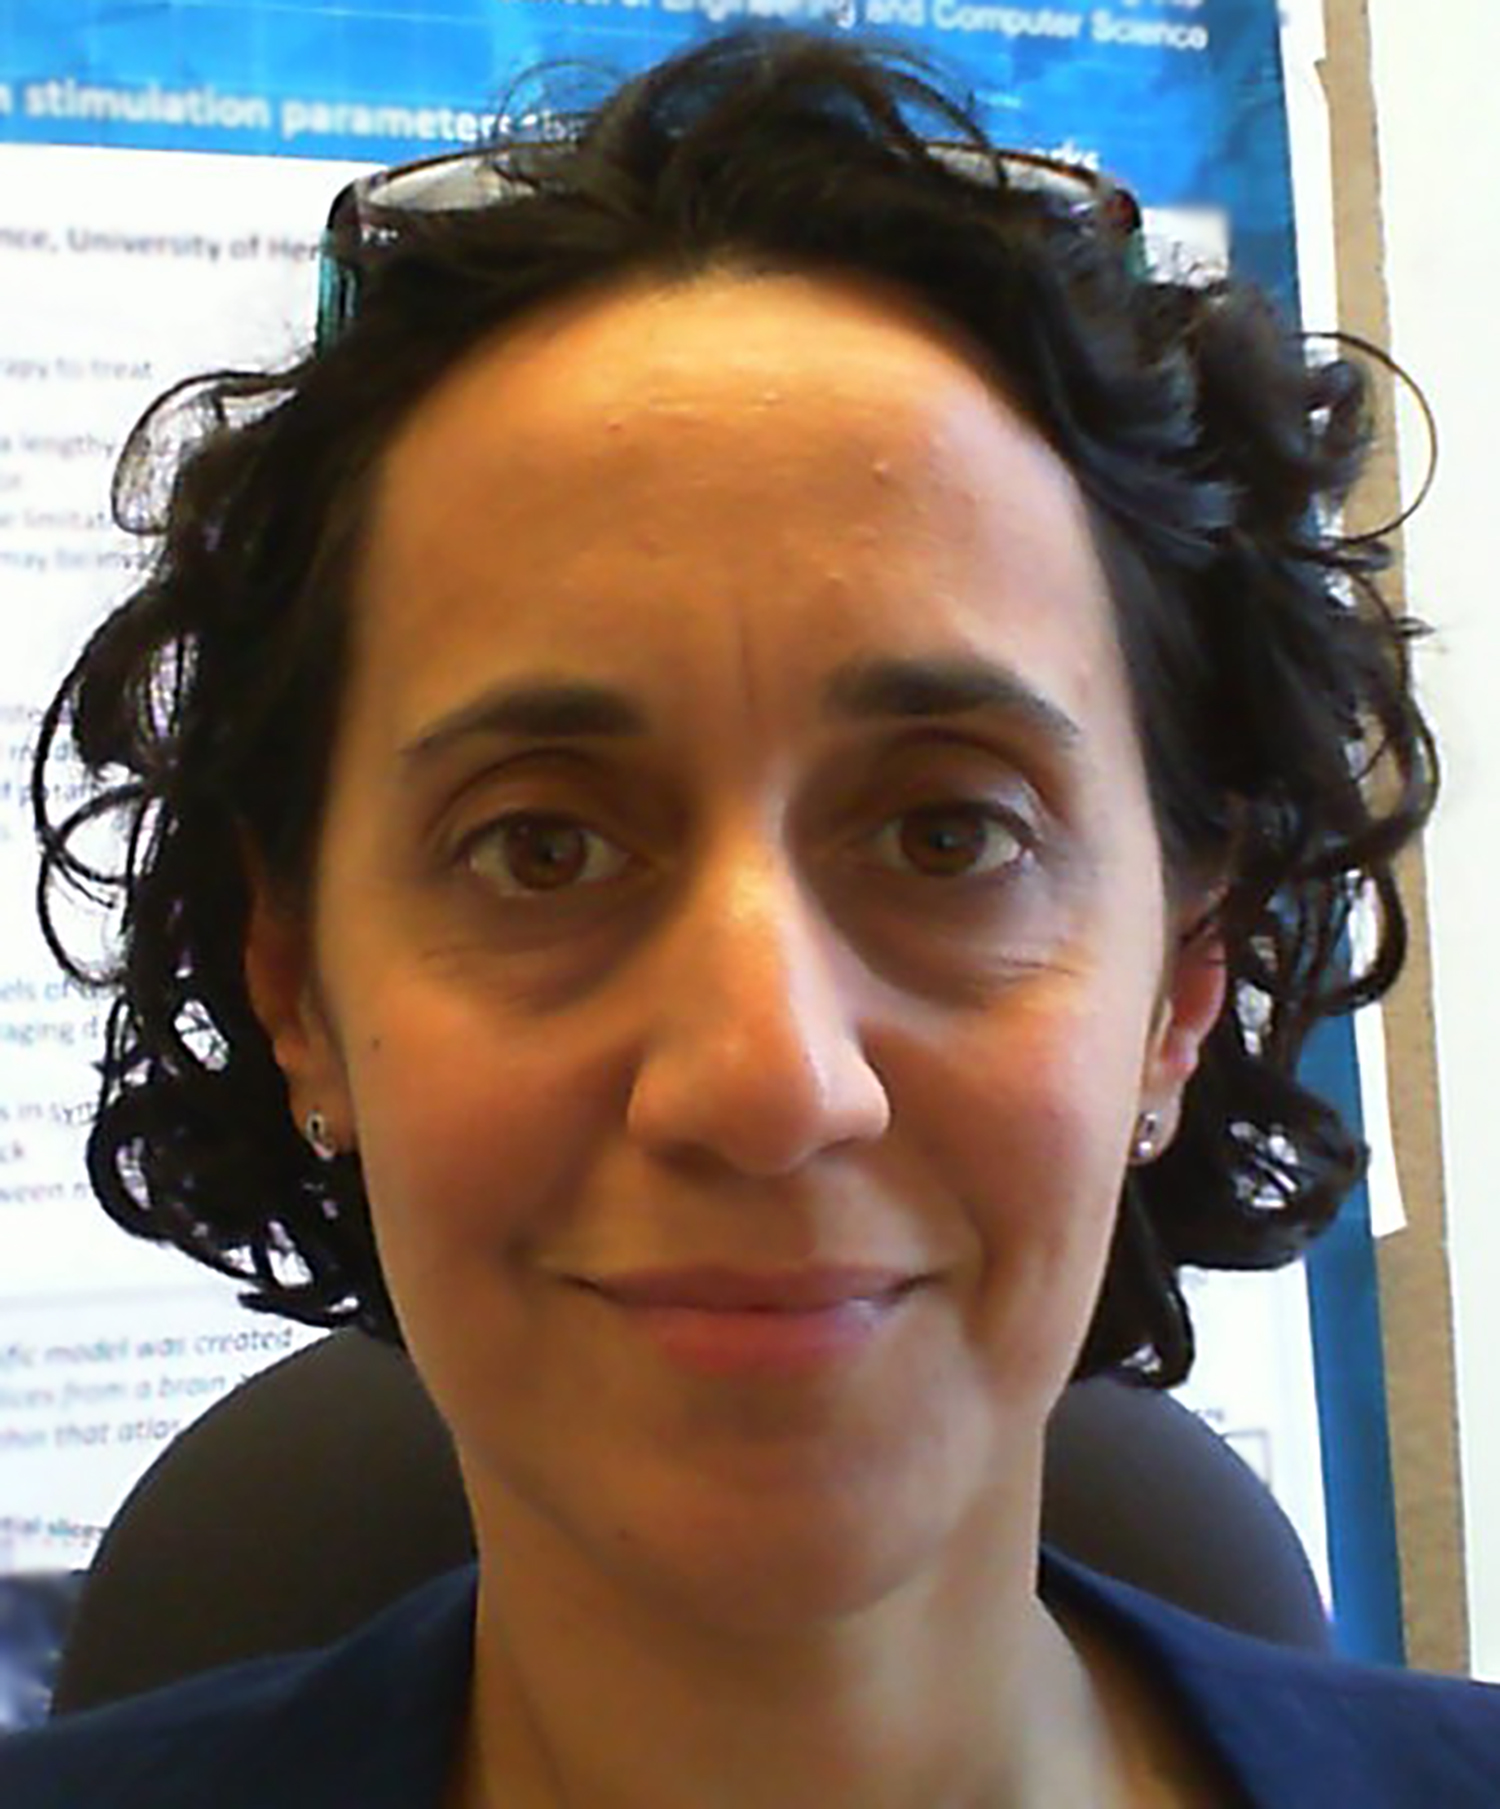
\includegraphics[height=16ex]{images/Yousif}\\
  \end{center}

  \vspace{1ex}
\textbf{Row 1}: Thomas Nowotny, Leonid Rubchinsky, Volker Steuber, Gennady Cymbalyuk, Julie Haas.\\
\textbf{Row 2}: Shailesh Appukuttan*, Roman Baravalle, Demian Battaglia, Alexander Dimitrov, Skirmantas Janusonis.\\
\textbf{Row 3}: Kerstin Lenk, Eirini Mavritsaki, Albert Mazzoni, Robert McDougal, Michelle Moerel.\\
\textbf{Row 4:} Adam Newton, Trang Anh Nghiem, Rodrigo de Oliveira Pena, Athanasia Papoutsi, Maurizio de Pitta.\\
\textbf{Row 5:} Cesar Renno-Costa, Ausra Saudargiene, Ankur Sinha*, Sergio Solinas, Nada Yousif.\\
(*Student/post-doc members)
\end{figure}
\vfill{}

\clearpage
\section*{OCNS Board:\ New arrivals and members rotating off}%
\sectionauthor{\vspace{-4ex}}


The current \href{https://www.cnsorg.org/board-of-directors}{Board of Directors} consists of 25 elected and ex officio members.
According to the \href{https://www.cnsorg.org/ocns-bylaws-2011}{OCNS Bylaws}, \href{https://www.cnsorg.org/election-procedures}{elections} are held to replace three or four outgoing directors each year.
The board elects its officers.
The duties carried out by members of the board can be seen \href{https://www.cnsorg.org/quick-director-duties}{here}.

\vspace{4ex}
\textbf{Terms for a number of Board members were renewed this year:}
\begin{multicols}{2}
  \begin{itemize}
    \item Thomas Nowotny (President)
    \item Leonid Rubchinsky (Vice president)
    \item Gennady Cymbalyuk (Treasurer)
  \end{itemize}
\end{multicols}

\textbf{The following members have completed their terms and have rotated off at the end of 2025.}
\textbf{OCNS thanks them for their service:}
\begin{multicols}{2}
  \begin{itemize}
    \item Max Garagnani (Sponsorship chair)
    \item Dimitros Pinotsis (Sponsorship chair)
    \item Tatiana Kameneva (Registration chair)
    \item Christopher French (Webmaster)
  \end{itemize}
\end{multicols}

\textbf{A number of new Board members were elected in the 2025 Elections, or have moved to new roles within the Board from 2026:}
\begin{multicols}{2}
  \begin{itemize}
    \item Maurizio de Pitta (Sponsorship chair)
    \item Skirmantas Janusonis (Registration chair)
    \item Roman Baravalle (Newsletter chair)
    \item Ausra Saudargiene (Social media chair)
    \item Nada Yousif (Training \& EDI chair)
    \item Cesar Renno-Costa (Travel awards chair)
    \item Trang Anh Nghiem (Membership chair)
    \item Adam Newton (Webmaster)
    \item Demian Battaglia (Workshops chair)
    \item Alexander Dimitrov (Tutorials chair)
  \end{itemize}
\end{multicols}

\clearpage
\section*{CNS*2025 Florence: in charts}%
\sectionauthor{%
  \hspace{-1ex}\begin{tabularx}{\textwidth}{lX}%
    Local Organizers: & Michele Migliore, Institute of Biophysics, Palmero, Italy\\
    & Sergio Solinas, University of Sassari, Sassari, Italy\\
    & Alessia Bonafede, Italian National Research Council, Italy
  \end{tabularx}}

  \textbf{Registrants (world):}
\begin{figure}[ht]
  \centering
  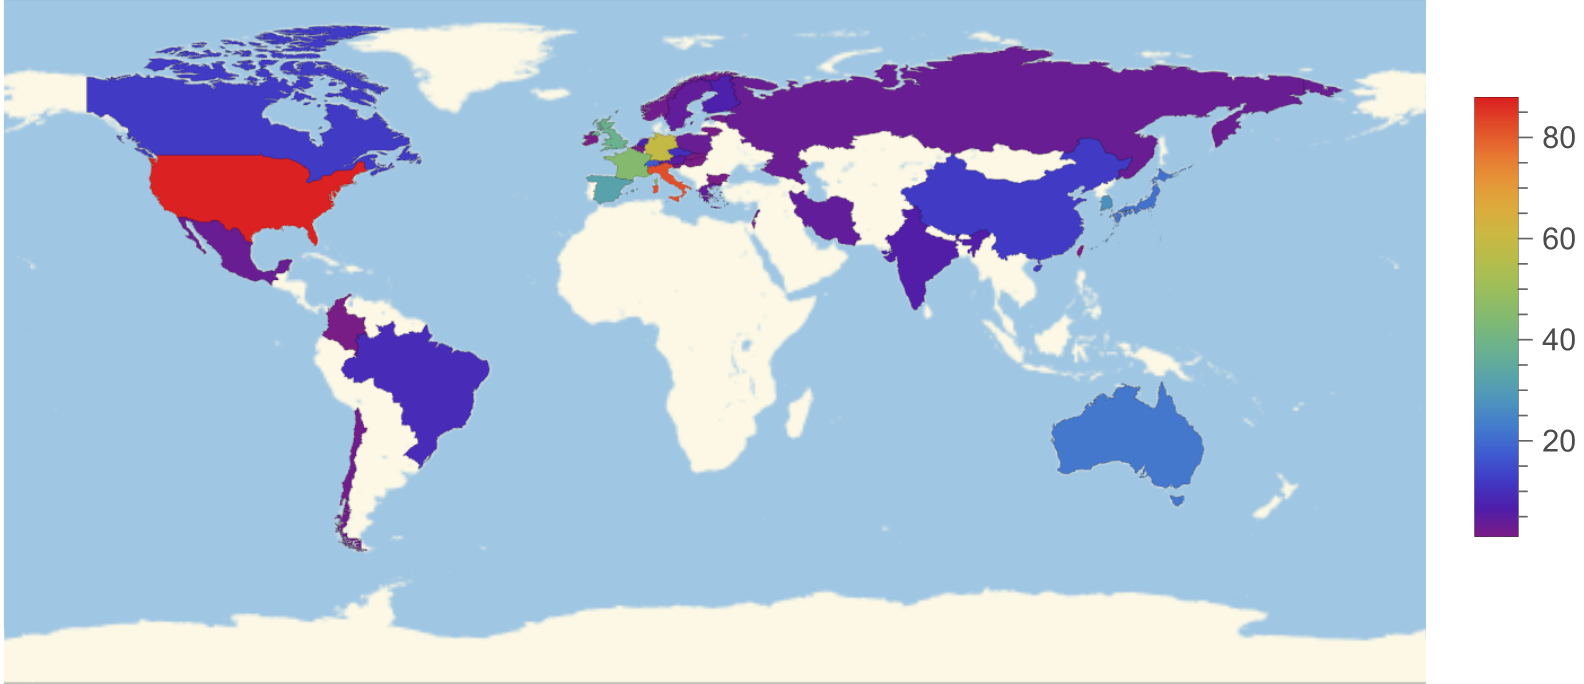
\includegraphics[width=0.9\textwidth]{images/cns2025-by-country-1}
\end{figure}

  \textbf{Registrants (Europe):}
\begin{figure}[ht]
  \centering
  \begin{subfigure}[c]{0.75\textwidth}
    \centering
  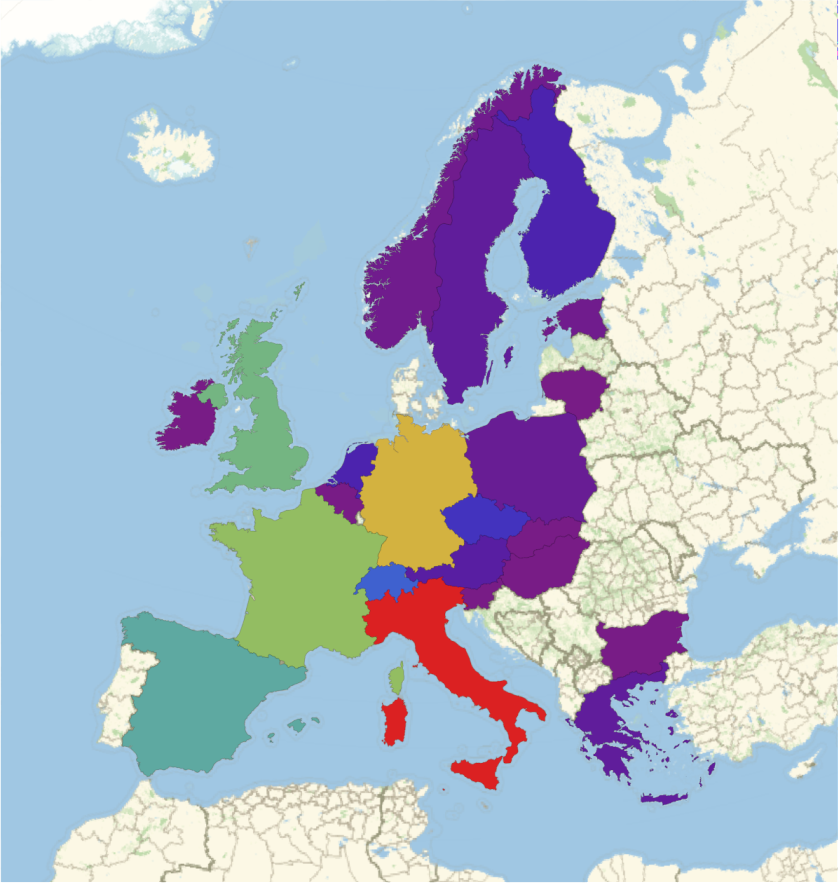
\includegraphics[width=0.8\textwidth]{images/cns2025-europeans-nolegend}
  \end{subfigure}
  \begin{subfigure}[c]{0.09\textwidth}
    \centering
  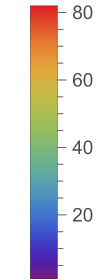
\includegraphics[width=\textwidth]{images/cns2025-europeans-legend}
  \end{subfigure}
\end{figure}
% to remove white background from the charts, use imagemagick:
% magick <input file> -fuzz 1%% -transparent White <output file>


\clearpage
\section*{CNS*2025 Florence: in charts}%
\sectionauthor{%
  \hspace{-1ex}\begin{tabularx}{\textwidth}{lX}%
    Vice President/Secretary: & Leonid Rubchinsky, Indiana University Indianapolis, USA\\
    Tutorials Chair: & Alberto Mazzoni, Krembil Research Institute, Toronto, Canada\\
    Workshops Chair: & Athanasia Papoutsi, Newcastle University, UK\\
    Infrastructure chair: & Christopher French, University of Melbourne, Australia\\
    Infrastructure chair: & Robert McDougal, University of Melbourne, Australia\\
    Treasurer: & Gennady Cymbalyuk, Georgia State University, USA\\
    Social Media Chair: & Claudio Mirasso, Universitat De Les Illes Balears, Spain\\
  \end{tabularx}}

  \textbf{Registrants (Asia):}
\begin{figure}[ht]
  \centering
  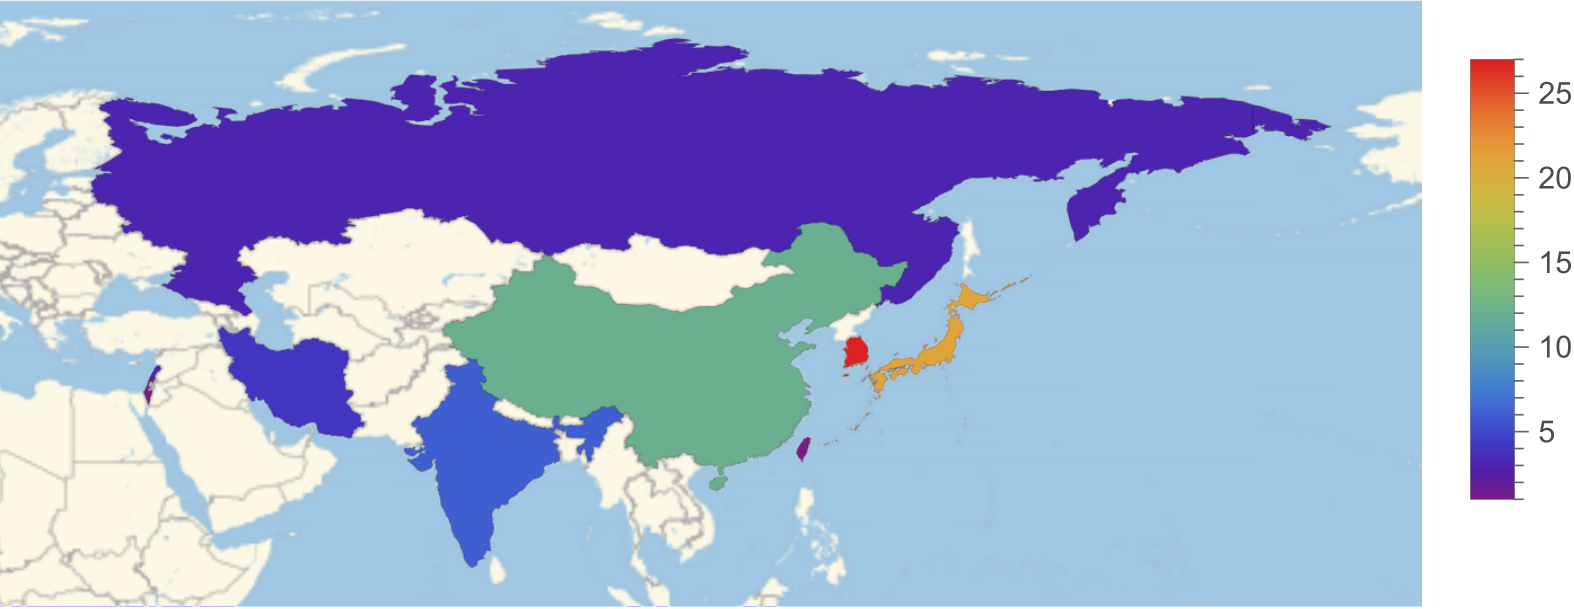
\includegraphics[width=0.9\textwidth]{images/cns2025-asia}
\end{figure}

  \textbf{Registrants (South America):}
\begin{figure}[ht]
  \centering
  \begin{subfigure}[c]{0.75\textwidth}
    \centering
  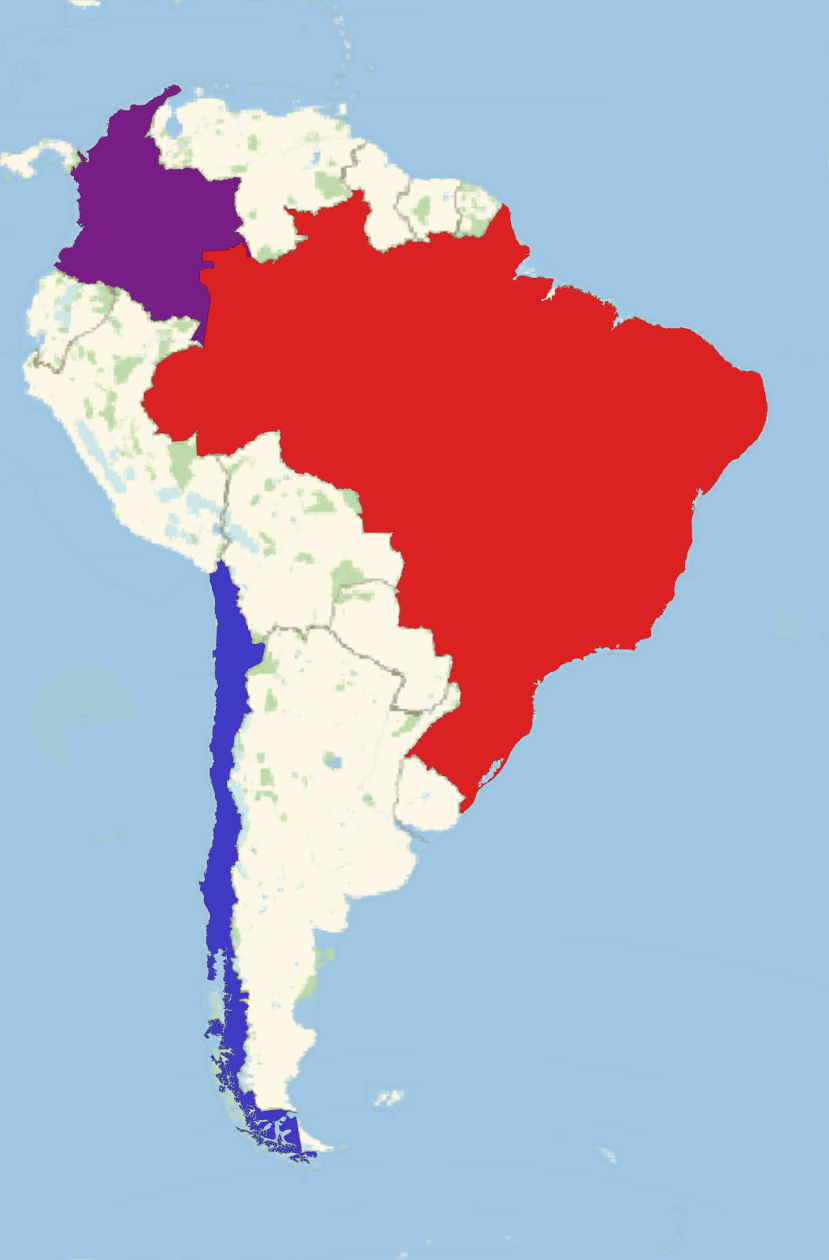
\includegraphics[width=0.6\textwidth]{images/cns2025-south-america-nolegend}
  \end{subfigure}
  \begin{subfigure}[c]{0.09\textwidth}
    \centering
  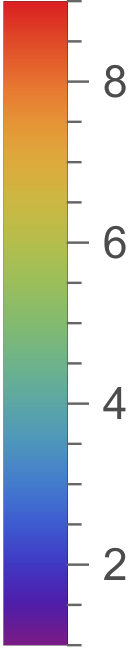
\includegraphics[width=0.7\textwidth]{images/cns2025-south-america-legend}
  \end{subfigure}
\end{figure}

\clearpage
\section*{CNS*2025 Florence: From the Program Chair}%
\sectionauthor{Program Chair:\ Julie Haas, Lehigh University, USA}
\begin{wrapfigure}[7]{l}{0.2\textwidth}
  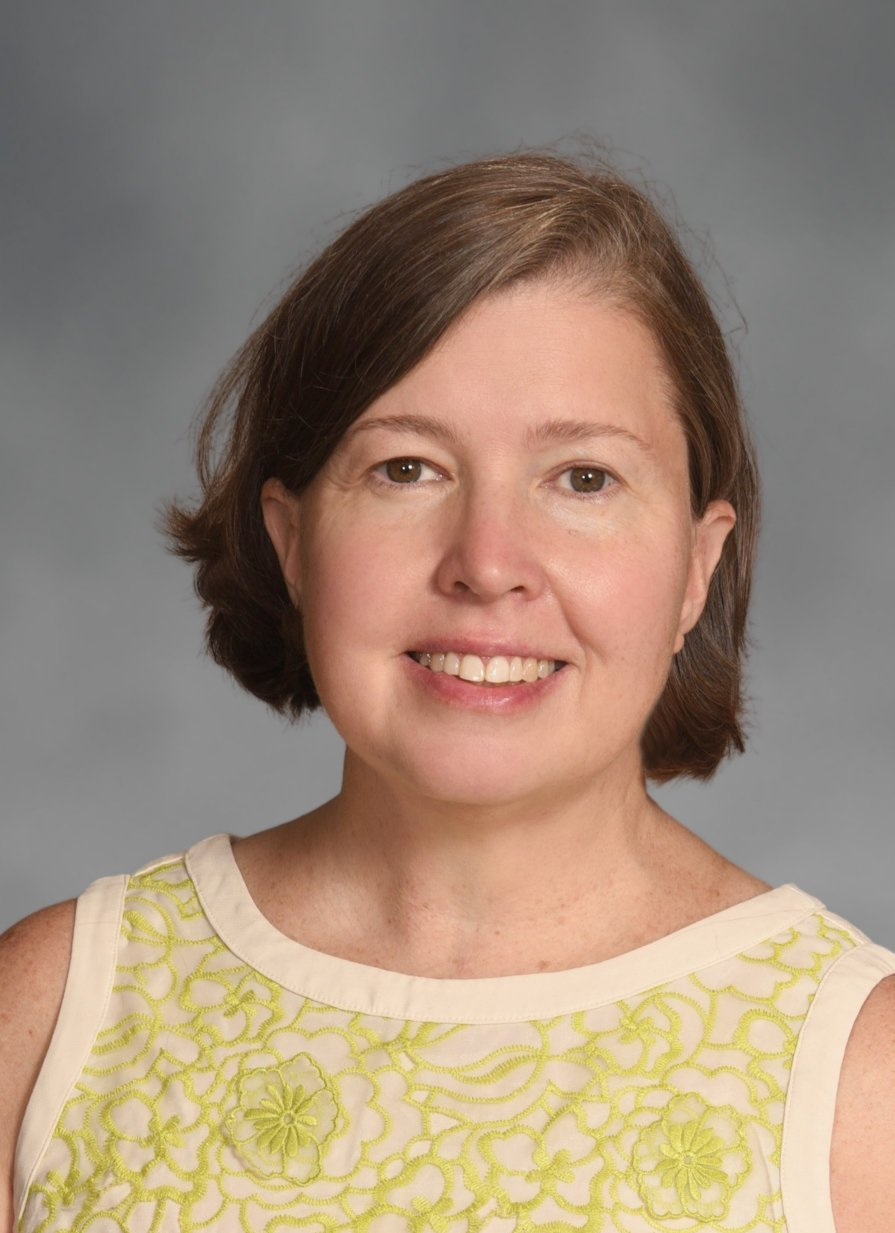
\includegraphics[width=0.2\textwidth]{images/Haas}
\end{wrapfigure}

Many thanks to departing members Amelie Aussel, Dai Feng Wang and Ilia Kuzneitsov.
This year we are excited to welcome Arezoo Alizadeh, Andre Peterson, Vasileios Christopoulos, Masanori Shimono, and Yunliang Zang who, along with the continuing members, have already selected a great slate of speakers for CNS*2026.
\vspace{15ex}
\input{travel-awards}

\iffalse
\clearpage
\section*{CNS*2025 Florence: Feedback form Summary}%
\sectionauthor{Registrations Chair:\ Tatiana Kameneva, Swinburne University of Technology, Australia}
\begin{wrapfigure}{l}{0.2\textwidth}
  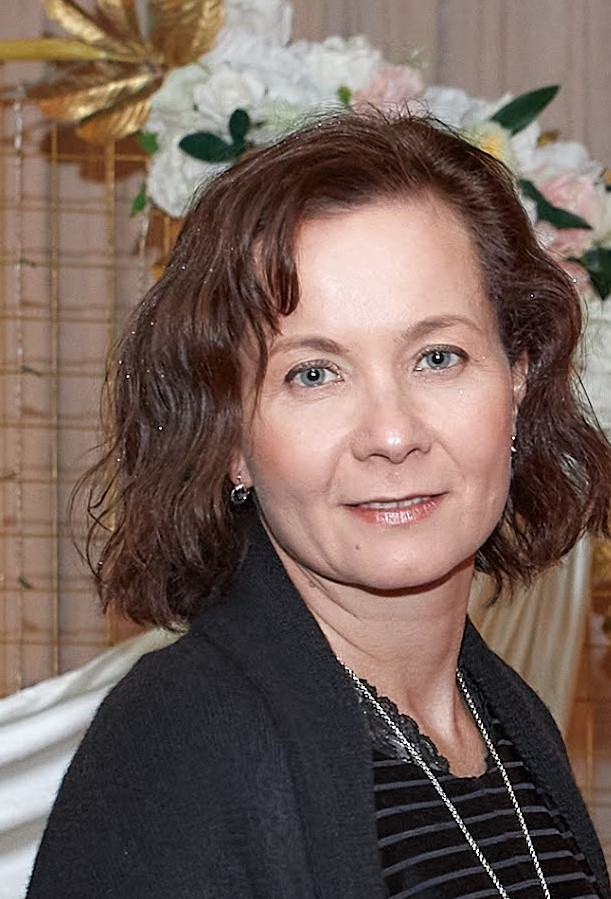
\includegraphics[width=0.2\textwidth]{images/Kameneva}
\end{wrapfigure}

We received 42 responses on the Participant Feedback Survey distributed at the end of CNS*2024.
Overall, the feedback has been positive. The data is presented in \cref{fig:cns2024-summary} above, with 5 being the highest rating.

Most people have enjoyed the venue: 71\% gave 4 or 5 rating in this category (\cref{fig:cns2024-summary} A).
Attendees commented highly on the quality of the keynote speakers: 55\% gave the highest (5) rating in this category (\cref{fig:cns2024-summary} B).
The common theme was a commendation to the local organizers for catering, efficiency, and airport pickup; while the AV, staff English proficiency, and the small space allocated for posters received mostly negative comments.

Tutorials had mixed reviews: 10\% of the attendees submitted the rating less than average satisfaction (1 or 2), while most people, 42\%, gave the rating 4 (\cref{fig:cns2024-summary} C). No comments were provided.

The attendance at the workshops varied.
Some workshops received very high praise; 80\% of people gave ratings 4 or 5, with comments such as \enquote{very interesting topics}, \enquote{amazing}, \enquote{excellent session} (\cref{fig:cns2024-summary} D).
While other workshops left attendees dissatisfied, with suggestions to reduce the number of parallel sessions to boost the attendance.

Overall, 79\% attendees enjoyed oral presentations and gave the ratings 4 or 5, while 21\% rated the presentation as satisfactory (3) or below (2), \cref{fig:cns2024-summary} E.
Positive comments included \enquote{OCNS is superb in supporting young scientist's careers}.
Suggestions for improvements included more talks on data-driven, deep learning-based approaches.
We thank everybody for their feedback that will be taken into account when organizing CNS*2025.

\begin{figure}[!h]
  \centering
  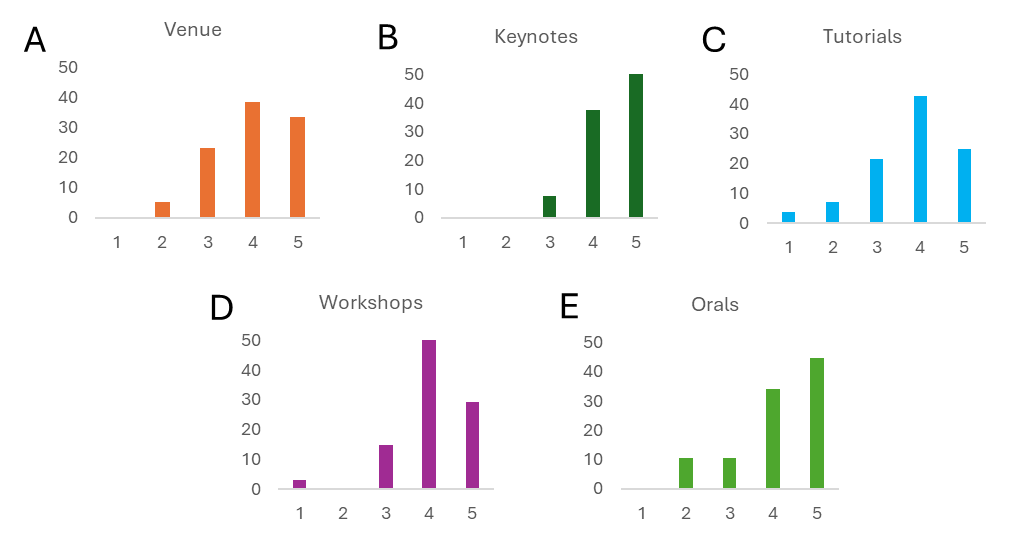
\includegraphics[width=\textwidth]{images/cns2024-feedback-form-summary}
  \caption{Summary of participant feedback, CNS*2024}%
  \label{fig:cns2024-summary}
\end{figure}

\fi
\clearpage

\section*{OCNS conference proceedings}%
\sectionauthor{Publications Chair:\ Shailesh Appukuttan, CRMBM \& INT, Aix-Marseille University, France}
\begin{wrapfigure}[8]{l}{0.2\textwidth}
  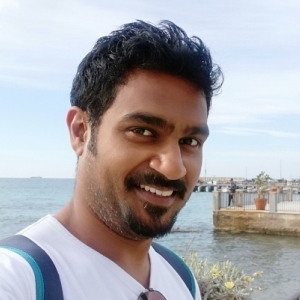
\includegraphics[width=0.2\textwidth]{images/Shailesh_Appukuttan_square}
\end{wrapfigure}

Proceedings from the annual CNS conferences are published by the end of the year annually.
Links to proceedings from previous conferences are below:
\begin{multicols}{2}
    \begin{itemize}
      \item \href{https://doi.org/10.1007/s10827-025-00892-8}{CNS 2024 Natal}\\(\href{https://doi.org/10.1007/s10827-025-00892-8}{Introduction})
      \item \href{https://link.springer.com/article/10.1007/s10827-024-00871-5}{CNS 2023 Leipzig}\\(\href{https://link.springer.com/article/10.1007/s10827-024-00872-4}{Introduction})
    \end{itemize}
\end{multicols}

Proceedings from previous conferences are archived on the website here:

\begin{center}
\url{https://www.cnsorg.org/annual-meeting-publications}.
\end{center}
\vspace{2ex}

\section*{OCNS Membership}%
\sectionauthor{Membership Chair: Rodrigo de Oliveira Pena, Florida Atlantic University, US}

The OCNS membership consists of:
\begin{table}[!h]
  \centering
  \begin{tabularx}{0.7\textwidth}{X|ccccc}
    \textbf{Member type}& \textbf{2025} & \textbf{2024} & \textbf{2023} & \textbf{2022} & \textbf{2021} \\
    \toprule{}
    Student & \textbf{228} & 139 &  185 & 182 & 212 \\
    Post-doc/not-for-profit employee & \textbf{137} & 93 & 135 & 118 & 141 \\
    Faculty/for-profit employee & \textbf{257} & 179 & 215 & 209 & 217 \\
    \midrule{}
    Total & \textbf{625} & 401 & 535 & 509 & 570 \\
  \end{tabularx}
\end{table}

\section*{Membership Benefits}%
\sectionauthor{\vspace{-4ex}}

OCNS members enjoy a number of rights and \href{https://www.cnsorg.org/member-benefits}{benefits}:
\begin{multicols}{2}
  \begin{itemize}
    \item Reduced conference registration fees
    \item Eligibility for travel awards
    \item Nomination and voting rights for OCNS director elections
    \item Special Interest Groups (SIGs)
    \item Computational neuroscience schools
    \item Submission of extra abstract to the conference
    \item Free access to Springer encyclopedia
    \item Reduced journal subscription fees
    \item Book discounts
  \end{itemize}
\end{multicols}

\section*{Membership Renewal}%
\sectionauthor{\vspace{-4ex}}

To \textbf{renew} your OCNS membership, please login at \href{www.cnsorg.org}{www.cnsorg.org} to pay your OCNS dues.
Please note that renewing with a multiple year membership will reduce your costs:

\begin{table}[!h]
  \centering
  \begin{tabularx}{0.7\textwidth}{X|ccc}
    \textbf{Member type}& \textbf{One year} & \textbf{Two years} & \textbf{Three years} \\
    \toprule{}
    Student & 10 USD & 15 USD & 20 USD \\
    Post-doc/not-for-profit employee & 20 USD & 30 USD & 40 USD \\
    Faculty/for-profit emplyoee& 50 USD & 75 USD & 100 USD \\
  \end{tabularx}
\end{table}

Please contact the Membership Chair at \href{mailto:membership@cnsorg.org}{membership@cnsorg.org} before you pay your dues if:
\begin{itemize}
  \item You are uncertain which category is appropriate for you.
  \item Your employment status has changed.
\item \emph{If you believe that special circumstances prohibit you from paying the full dues.}
\end{itemize}

\vspace{1ex}
\centerline{\rule{0.5\textwidth}{0.4pt}}
\vspace{1ex}
Membership type definitions:
\begin{itemize}
  \item \textbf{Student:} Anybody studying toward an undergraduate or graduate degree.
  \item \textbf{Postdoc/not-for-profit employee:} Anybody who is employed as a postdoctoral scholar or postdoctoral fellow, and anybody who is employed in a university lab or non-industry research institute as a technician or research assistant not seeking a degree.
  \item \textbf{Faculty/for-profit employee:} Anybody who is employed as faculty, laboratory head, independent researcher, or in an equivalent position, and anybody who is employed in industry or for-profit institutions
  \item Retired persons should apply for or remain in their pre-retirement category.
\end{itemize}


\clearpage
\section*{Frontiers in Computational Neuroscience partnership}%
\sectionauthor{\vspace{-4ex}}

\textbf{Submit a Research Topic idea to Frontiers in Computational Neuroscience}

Are you passionate about a specific area of computational neuroscience?
Submit your idea and become a Topic Editor of an OCNS Research Topic---a collaborative article collection hosted by Frontiers in Computational Neuroscience.

\vspace{1ex}
\centerline{\rule{0.5\textwidth}{0.4pt}}
\vspace{1ex}
\textbf{Who can become a Topic Editor?}

Researchers who have completed a PhD are eligible to edit a Research Topic in Frontiers in Computational Neuroscience.
If you have not completed a PhD but are interested in a Topic Coordinator role, you are also welcome to complete this form.
The role is similar to a Topic Editor position, but you will not handle manuscripts during peer review.

\vspace{1ex}
\centerline{\rule{0.5\textwidth}{0.4pt}}
\vspace{1ex}
\textbf{Why host a Research Topic?}

By leading one of our expert-led article collections, you will benefit from:

\begin{itemize}
  \item A free editorial article
  \item A full APC waiver dedicated to your Research Topic (specific advantage if you edit an OCNS society led collection)
  \item Networking and collaboration with experts in your field
  \item A downloadable e-book summarizing your Topic (when 10+ articles are published)
\end{itemize}

We are especially keen to receive proposals from OCNS members who want to help advance the field of computational neuroscience.

\vspace{1ex}
\centerline{\rule{0.5\textwidth}{0.4pt}}
\vspace{1ex}
\textbf{Please use the link below to submit a topic:}

\begin{center}
\begin{tcolorbox}[colback=lighterOrange, colframe=black, width=\textwidth, boxrule=0.1mm]
\begin{center}
  \href{https://url.uk.m.mimecastprotect.com/s/j360CQ5WAhVr7MLTxfLIG_wZD?domain=forms.gle}{https://url.uk.m.mimecastprotect.com/s/j360CQ5WAhVr7MLTxfLIG\_wZD?domain=forms.gle}
\end{center}
\end{tcolorbox}
\end{center}

\clearpage
\iffalse{}
\section*{Initiatives: Software Working Group}%
\sectionauthor{Co-chairs: Marcel Stimberg, Sorbonne Universite, Paris, France\\
\phantom{Co-chairs: }Ankur Sinha, University College London, UK}
\begin{wrapfigure}{l}{0.2\textwidth}
  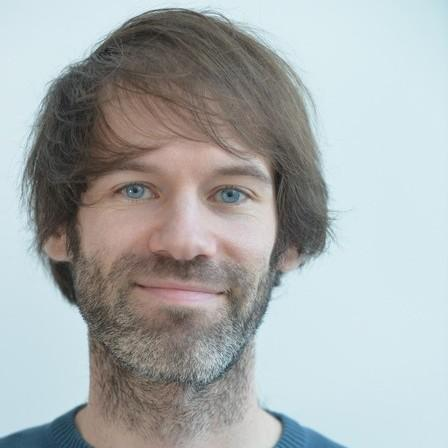
\includegraphics[width=0.2\textwidth]{images/marcel}
  
\includegraphics[width=0.2\textwidth]{images/ankur-sinha}
\end{wrapfigure}

The Software Working Group aims to increase awareness and knowledge of the various software tools that we use to carry out our research.
The group is an open community group that everyone is welcome to join.
It is shared between the OCNS and the \href{https://incf.org}{International Neuroinformatics Co-ordinating Facility (INCF)}, of which OCNS is a member organization.

In the past year, the group has continued to host sessions on different neuroscience software.
Recordings from these sessions can be found on the \href{https://www.youtube.com/@IncfOrg_INCF/videos}{INCF YouTube channel}, and also on the \href{https://training.incf.org/course/incfocns-working-group-computational-neuroscience-software}{INCF Training Space}.
Working group announcements are published on our \href{https://ocns.github.io/SoftwareWG/}{website}.

If there are software tools/standards that you think are useful for the community to know and learn about, please contact either of the working group co-chairs to let us know (\href{mailto:marcel.stimberg@sorbonne-universite.fr}{marcel.stimberg@sorbonne-universite.fr}, \href{mailto:ankur.sinha@ucl.ac.uk}{ankur.sinha@ucl.ac.uk}).
We will reach out to the developers of the software to organize a session on it.

The working group also sets up task forces to work on specific projects.
Currently, a task force is working on developing a simple web based tool to help community members decide what simulation tool they should use.
A working title for this tool is \href{https://github.com/OCNS/simselect/issues}{Simselect}. 
If you would like to get involved in this task force, please let us know.

\section*{Initiatives: Mentoring Scheme}%
\sectionauthor{EDI Chair: Eirini Mavristaki, Birmingham City University, UK}
\begin{wrapfigure}[9]{r}{0.2\textwidth}
  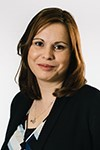
\includegraphics[width=0.2\textwidth]{images/Mavritsaki}
\end{wrapfigure}

OCNS is currently working on a mentorship scheme for members.
The scheme aims to provide support to members to develop their research careers further to move to the next level of their professional development.
It aims to provide the space for our researchers to be supported and through this to identify areas that we could develop to be able to support our community more.

More details on the OCNS mentoring scheme will be announced shortly.
Please do keep an eye out for related communications and please do get in touch (\href{mailto:eirini.mavritsaki@bcu.ac.uk}{eirini.mavritsaki@bcu.ac.uk}) if you would like to help in its organization.

\vspace{7ex}
\section*{Initiatives: OCNS Job Board}%
\sectionauthor{\vspace{-4ex}}

A \textbf{new} OCNS Job Board is now live at \url{https://www.cnsorg.org/job-board}.
Please use the form provided to submit jobs openings and bookmark the page for updates.

\clearpage
\fi{}
\input{incf.tex}

\clearpage
\section*{Neuromatch}%
\sectionauthor{Enabling inclusinve collaborative and global participation in the computational sciences}

\begin{figure}[!h]
  \centering
  
\includegraphics[width=0.8\textwidth]{images/neuromatch-logo-2-transparent}
\end{figure}

Neuromatch is a nonprofit organization (registered as a 501(c)(3) in the U.S.) training the next generation of global computational research leaders.

\section*{Neuromatch Academy}
\sectionauthor{\vspace{-4ex}}

Applications for our Neuromatch Academy open 16 February until 15 March.
Neuromatch run virtual courses in Computational Neuroscience, NeuroAI, Deep Learning, and Computational Tools for Climate Science in July.
More information at: \href{https://neuromatch.io/courses/}{https://neuromatch.io/courses/}.
\vspace{1ex}

\begin{figure}[!h]
  \centering
  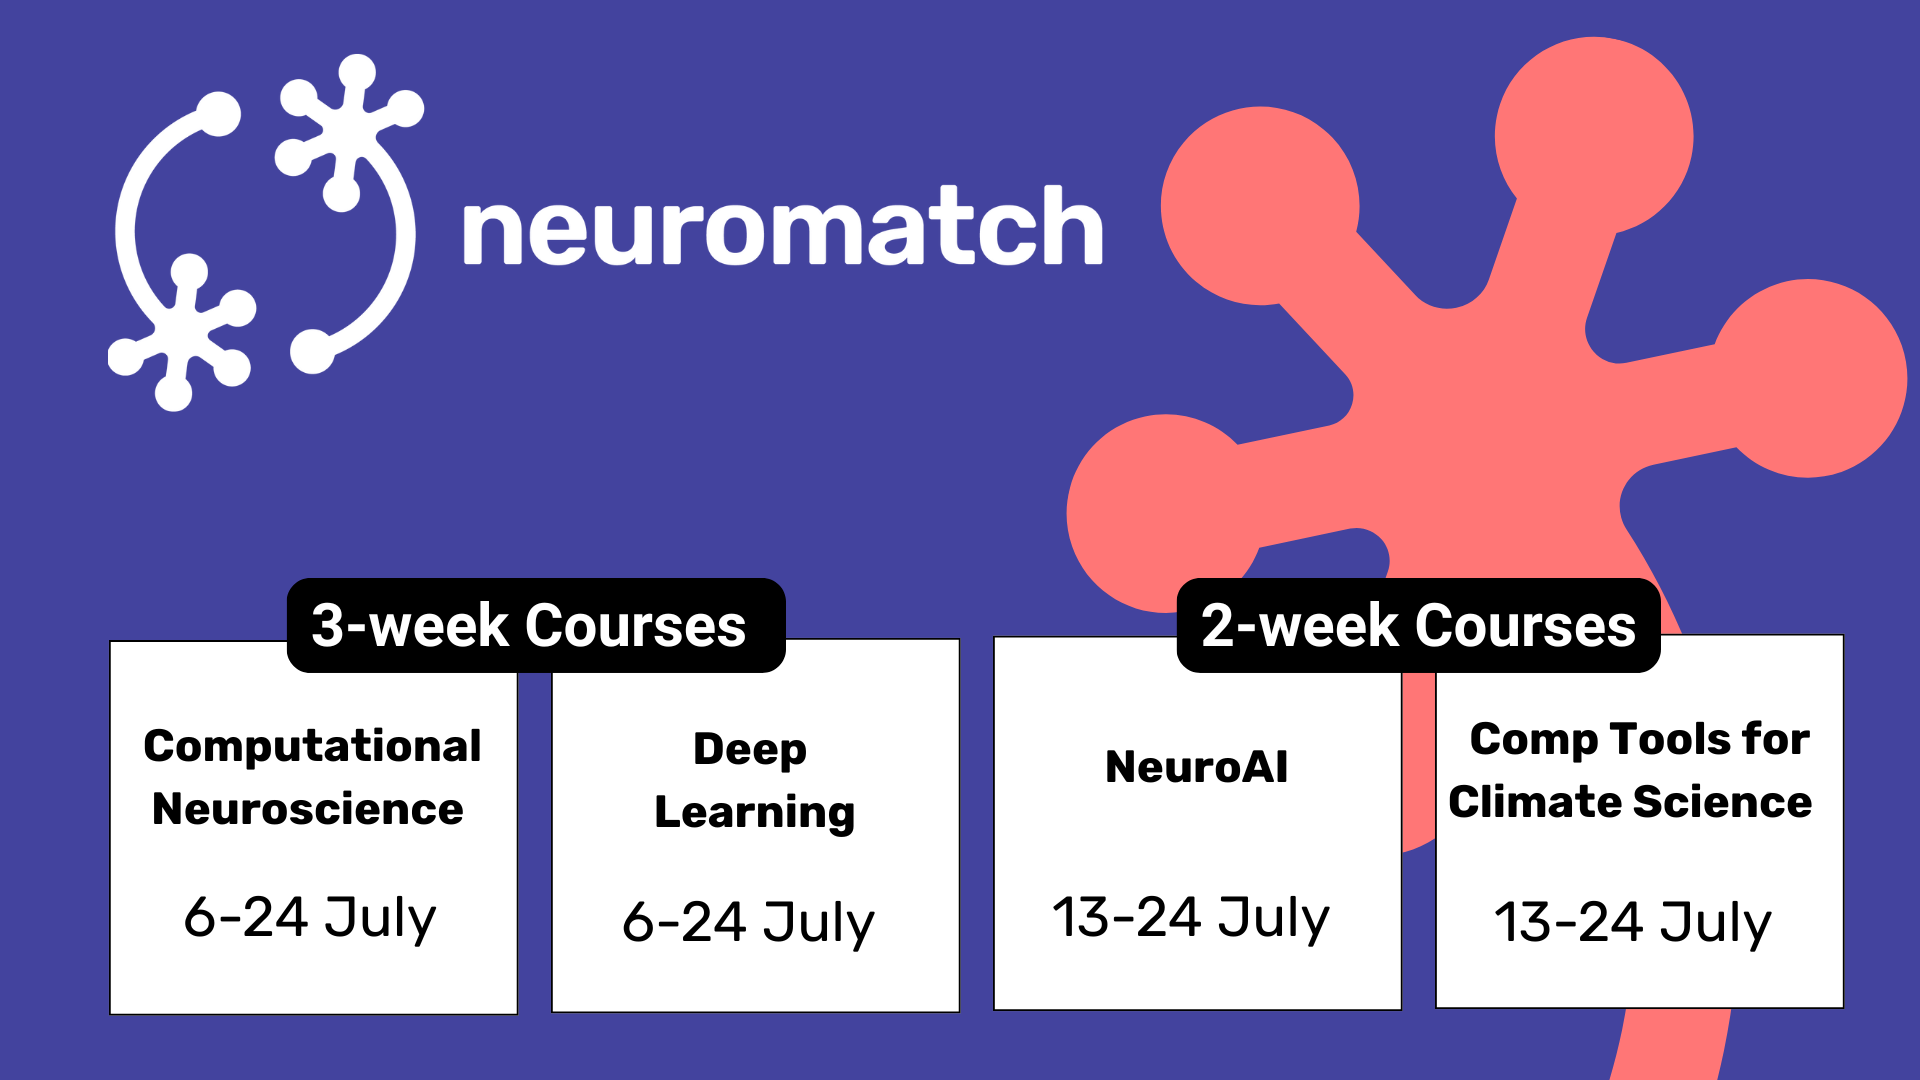
\includegraphics[width=0.8\textwidth]{images/2026-nma}
\end{figure}

\section*{Connect with Neuromatch}
\sectionauthor{\vspace{-4ex}}
\vspace{1ex}
\begin{center}
  \href{https://twitter.com/neuromatch?lang=en}{\vcenteredinclude{./images/X-logo}}~
  \href{https://www.facebook.com/Neuromatch/}{\vcenteredinclude{./images/Facebook_icon_2013.svg}}~
  \href{https://neuromatch.social/@neuromatch}{\vcenteredinclude{./images/mastodon}}~
  \href{https://www.linkedin.com/company/neuromatch}{\vcenteredinclude{./images/LinkendIn}}~
  \textbf{\Large @Neuromatch}
\end{center}
\vspace{1ex}


\clearpage
\iffalse{}
\input{member-updates.tex}
\input{member-updates-community.tex}
\clearpage
\fi{}
\section*{Support OCNS}%
\sectionauthor{
  \hspace{-1ex}\begin{tabularx}{\textwidth}{lX}%
    Sponsorship Chairs: & Maurizio de Pitta, University of Toronto, Canada\\
  \end{tabularx}}%
\begin{wrapfigure}[16]{l}{0.2\textwidth}
  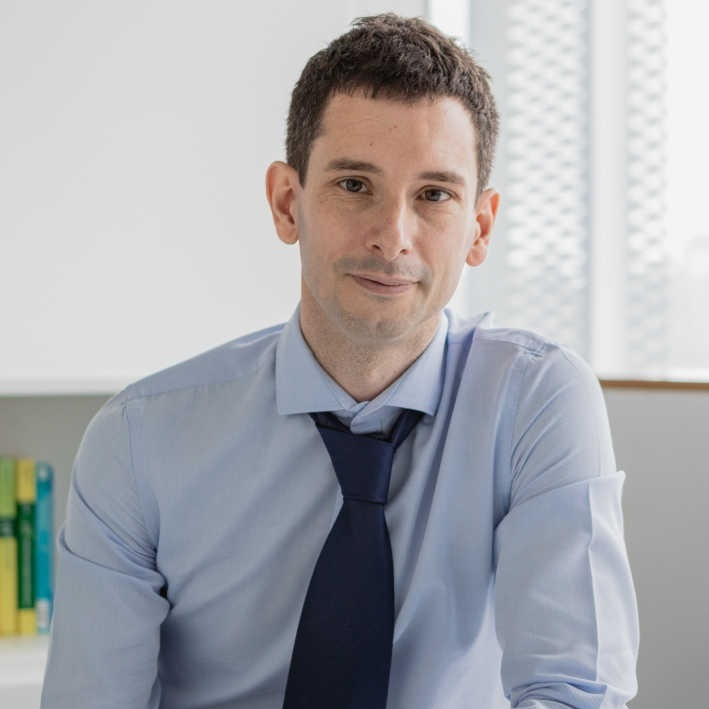
\includegraphics[width=0.2\textwidth]{images/Pitta}
\end{wrapfigure}

OCNS is a non-profit organization supporting the international computational neuroscience community.
Our annual meetings draw \textasciitilde{}500 attendees from a variety of backgrounds: physics, mathematics, computer science, biology, medicine, engineering, and others.
We seek sponsorship from corporate and philanthropic organizations to support the annual OCNS meeting.
We have predefined levels of sponsorship and are also happy accommodate specific requests:

\begin{multicols}{2}
    \begin{itemize}
      \item \textbf{Silver: USD 2000}
      \item \textbf{Gold: USD 3000}
      \item \textbf{Platinum: USD 5000}
    \end{itemize}
\end{multicols}

Sponsor names and logos with links to sponsor websites will be featured in the program and on the OCNS website.
Sponsors may also send attendees to the meeting.
These attendees will have access to the main meeting, the conference banquet, and workshops at no cost for Gold and Platinum level sponsorships.
Gold and Platinum level sponsors may also host booths in central meeting foyer or provide leaflets and posters to be displayed.

\vspace{4ex}
Additional opportunities for specific acknowledgements may include (we will work with you to create a suitable package):
\begin{multicols}{2}
    \begin{itemize}
      \item  Advertisements in the program.
      \item  Sponsorship of a specific plenary talk or specific session.
      \item Sponsorship of a specific workshop or tutorial.
      \item  Sponsorship of the banquet.
    \end{itemize}
\end{multicols}

Past sponsors include MetaCell, MathWorks, Springer Nature, BrainCorp, Neuralynx, CRC Press, Bernstein Network, eLife, Frontiers, INCF, NSF, MIT Press, and many others.

\vspace{1ex}
\centerline{\rule{0.5\textwidth}{0.4pt}}
\vspace{1ex}

We also seek financial support through \textbf{donations and endowments} from individuals and corporations to promote computational neuroscience around the world.
You may make a private donation by check to our \href{https://www.cnsorg.org/all-contacts}{mailing address}, directed to the OCNS Treasurer.
If you would like to discuss how you can contribute differently or to target a donation, please contact the OCNS President directly.

\vspace{1ex}
\centerline{\rule{0.5\textwidth}{0.4pt}}
\vspace{1ex}

OCNS is a 501(c)(3) non-profit/charitable organization registered in the USA.
Sponsorship is tax-deductible to the extent provided by the US tax laws.
Gifts and contributions can be deducted except for the amount of waived registration fee.

\vspace{3ex}
\begin{center}
\begin{tcolorbox}[colback=lighterOrange, colframe=black, width=0.7\textwidth, boxrule=0.1mm]
\begin{center}
Please contact the Sponsorship Chairs at \href{mailto:sponsorship@cnsorg.org}{sponsorship@cnsorg.org} for information on \href{https://www.cnsorg.org/support-ocns}{supporting OCNS}.
\end{center}
\end{tcolorbox}
\end{center}


\clearpage

\vspace{5ex}
\begin{figure}[!h]
  \centering
  
\includegraphics[width=0.8\textwidth]{images/Metacel_logo_2_crop}
\end{figure}

Thank you to OCNS for hosting an excellent annual meeting, and to everyone who connected with MetaCell, attended our presentation and joined our event.
It was great catching up with friends and partners in Natal, and we were proud sponsors of the meeting!

If you're interested in new ways to standardize, visualize, share, and build your computational models, please visit \url{metacell.us} and get in touch with our team.

\vspace{5ex}
\centerline{\rule{0.5\textwidth}{0.4pt}}
\vspace{5ex}
\begin{center}
  \begin{minipage}{\textwidth}
    \begin{center}
      Copyright \textcopyright{} OCNS 2026.\\\vspace{2ex}

      The OCNS newsletter is distributed under the \href{https://creativecommons.org/licenses/by-nc-nd/4.0/}{CC By-NC-ND} license.\\\vspace{2ex}

      Please contact the Newsletter Chair, Ankur Sinha, at \href{mailto:newsletter@cnsorg.org}{newsletter@cnsorg.org} for any contributions, corrections, clarifications, comments, and remarks.
    \end{center}
  \end{minipage}
\end{center}
\vfill
\clearpage
\end{document}

